Selon le fait \ref{nece-cond}, si parmi les \ngones\ de périmètre fixé, il en existe un qui maximise l'aire, alors ce ne peut être que le \ngone\ régulier. Nous allons établir que cette condition nécessaire est suffisante. Pour cela, nous avons juste besoin de savoir qu'il existe au moins un \ngone\ d'aire maximale.
Comme dans la remarque \ref{tri-topo-comp}, nous allons convier le couple continuité/compacité, mais ici les choses se compliquent, car nous allons devoir accepter de travailler avec des polygones croisés, et par conséquent il nous faut un moyen de mesurer la surface de tels polygones (le vrai point délicat est ici). 
Plaçons-nous d'un point de vue informatique: comme on sait calculer l'aire d'un triangle via le calcul d'un déterminant,%
\footnote{
	Il est connu que $\area{ABC} = \dfrac12 \abs{\det \big( \vect{AB} , \vect{AC} \big)}$.
}
il est naturel de chercher à calculer l'aire d'un \ngone\ en utilisant des triangles.
Voici une méthode possible où l'usage du déterminant pour calculer les aires des triangles à partir de coordonnées de vecteurs fait apparaître des signes moins. On obtient alors l'aire géométrique à un signe près. A priori, le résultat dépend du point $\Omega$ employé, mais le fait \ref{garea-pt-ct}, donné plus bas, montrera que ce n'est pas le cas.

\begin{multicols}{2}
	\small\itshape
    \begin{center}
		Calcul direct à la main.
		
		\smallskip
		
        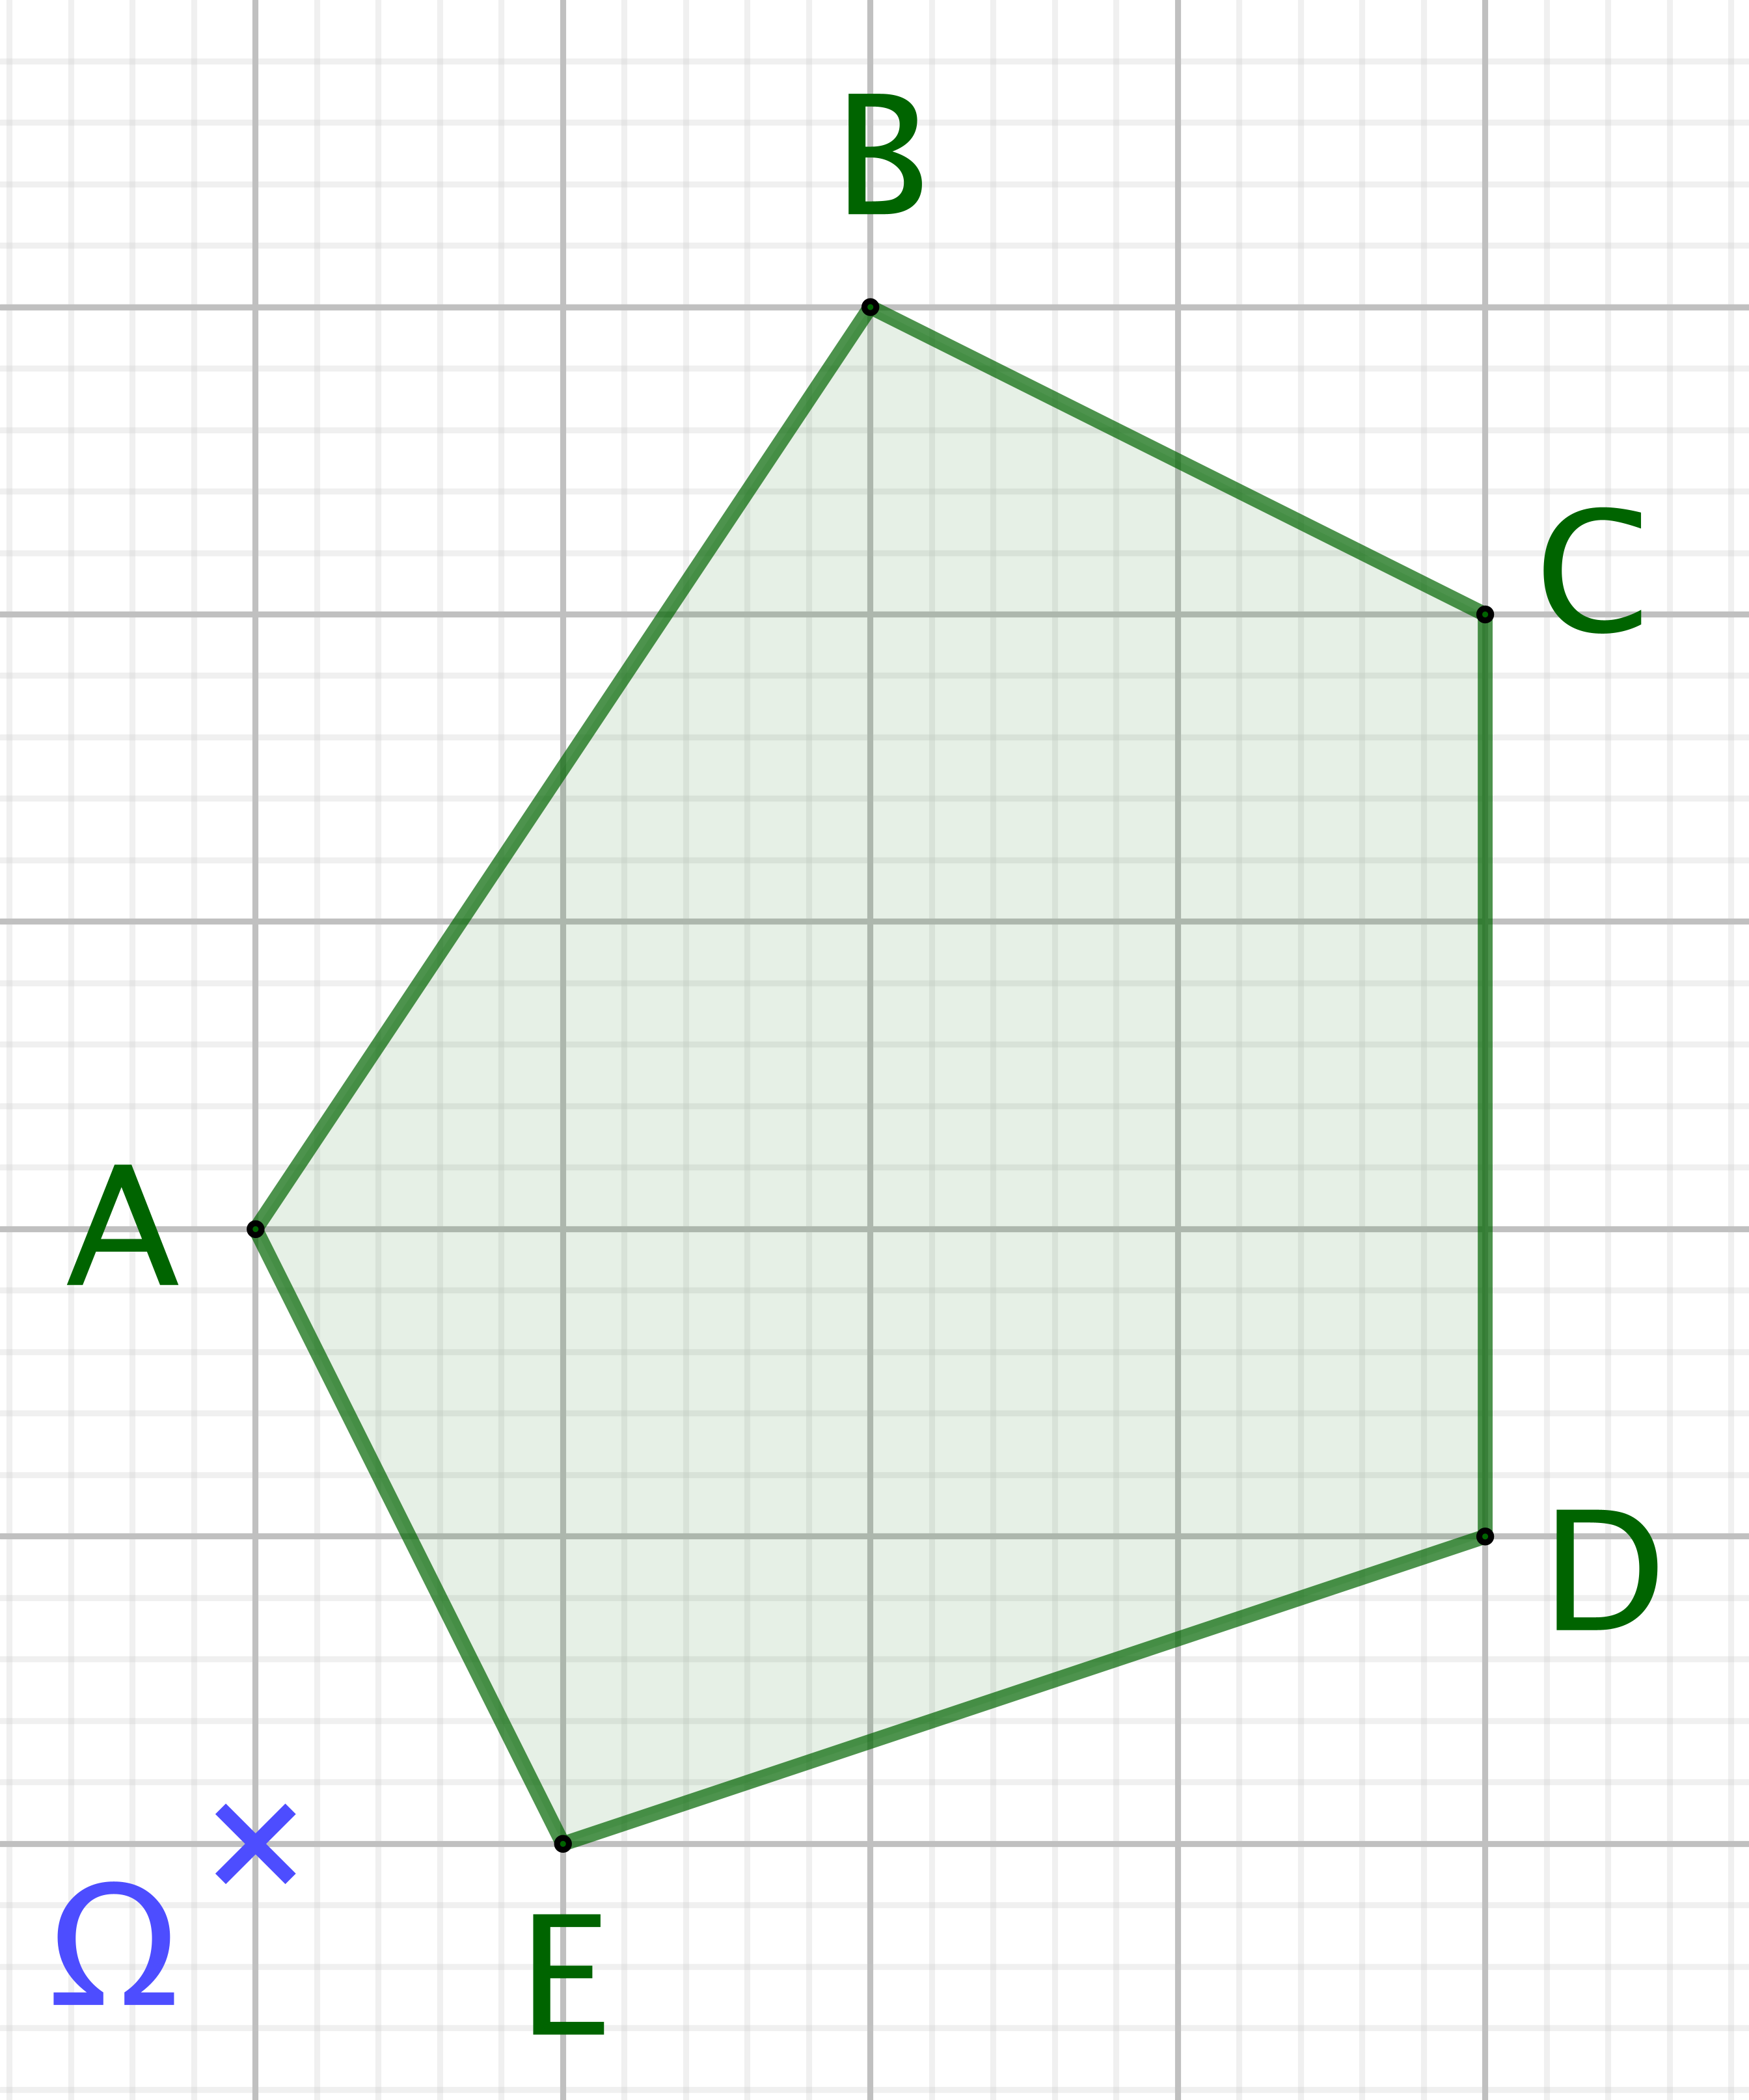
\includegraphics[scale=.4]{content/polygon/sufficient-cond/convex-1.png}
        
       	\smallskip
	
		$\num{14.5} = 4 \cdot 6 - \dfrac{2 \cdot 4 + 2 \cdot 1 + 3 \cdot 2 + 1 \cdot 3}{2}$
    \end{center}

	\columnbreak
	
    \begin{center}
		Via le déterminant.

		\smallskip
		
        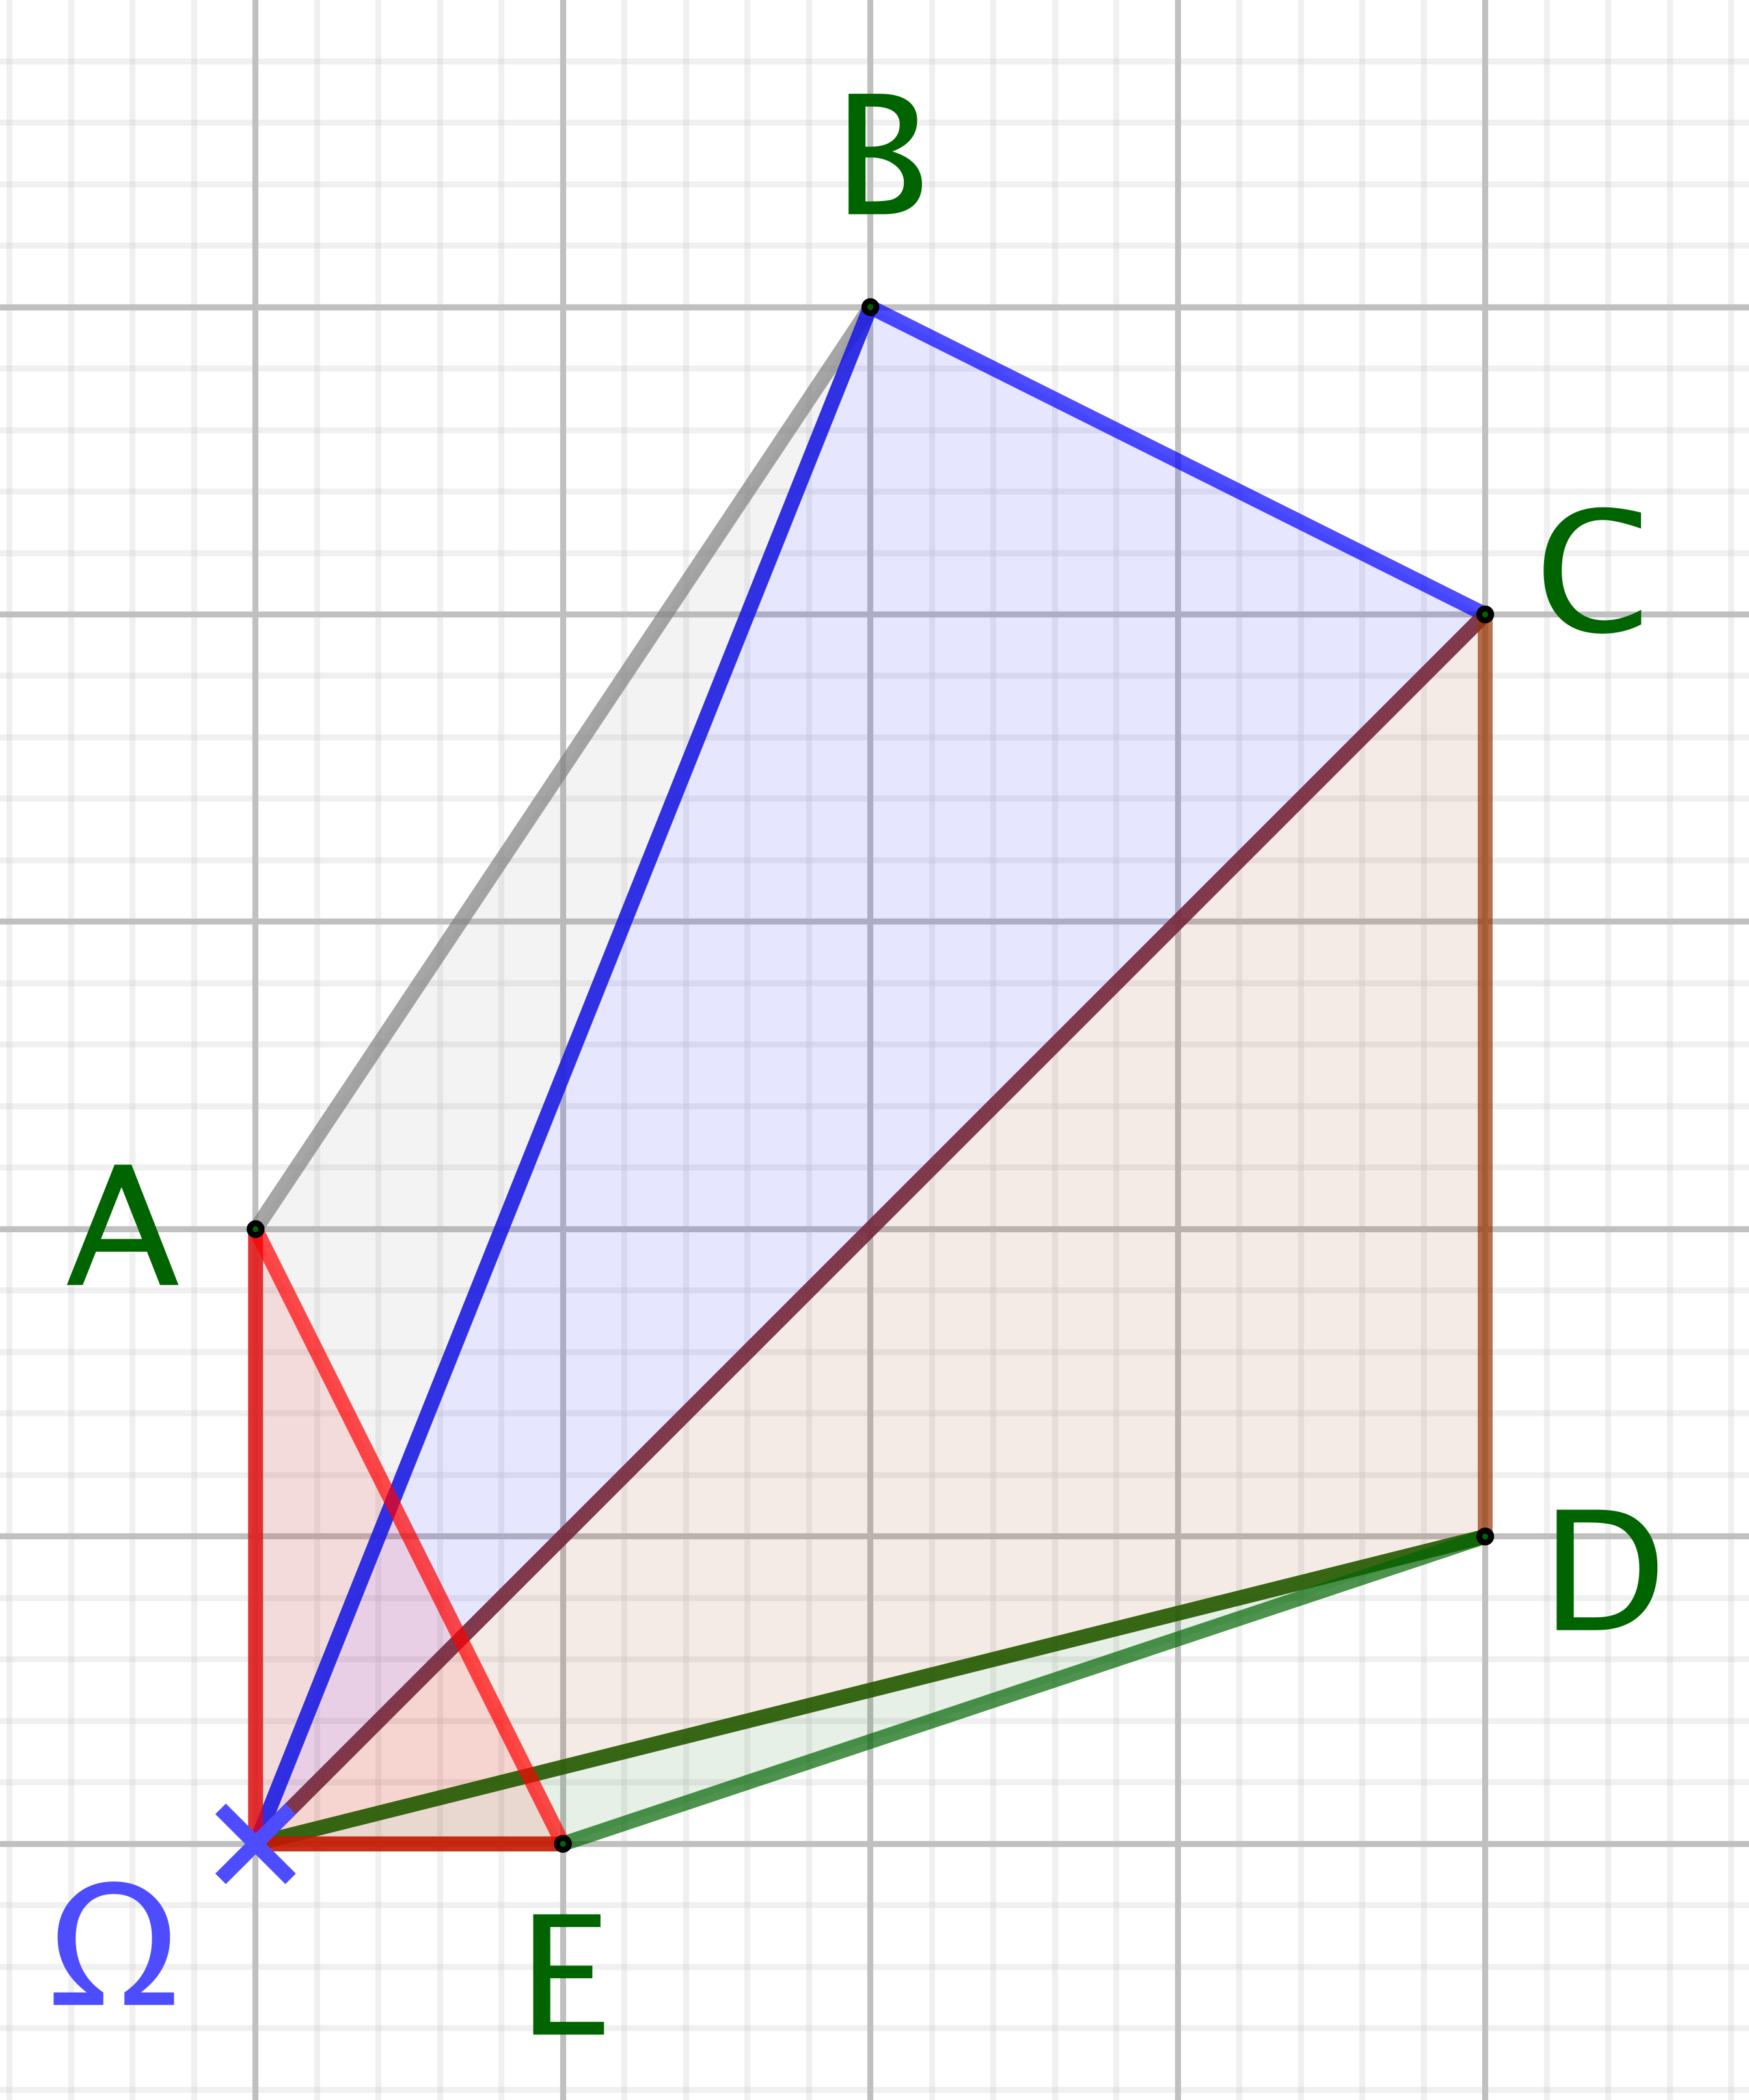
\includegraphics[scale=.4]{content/polygon/sufficient-cond/convex-2.png}
        
       	\smallskip
	
		$- \num{14.5} = -2 - 7 - 4 - \num{4.5} + 3 \vphantom{\dfrac22}$
    \end{center}
\end{multicols}


Ce mode de calcul est celui employé par \geogebra\ qui donne une aire de \num{6.5} pour le polygone croisé de la bande dessinée ci-après qui détaille les calculs faits: les aires algébriques représentées en bleu sont positives, et celles en rouge négatives.
Nous obtenons un total de $( - \num{6.5})$, soit, de nouveau, la valeur fournie par \geogebra\ au signe près.
L'apparition du signe moins dans ce cas et le précédent vient en fait du sens horaire de parcours des polygones comme nous le montrera le fait \ref{route-direction}.

%\newpage

\begin{multicols}{3}
    \small\itshape
    
    \begin{center}
        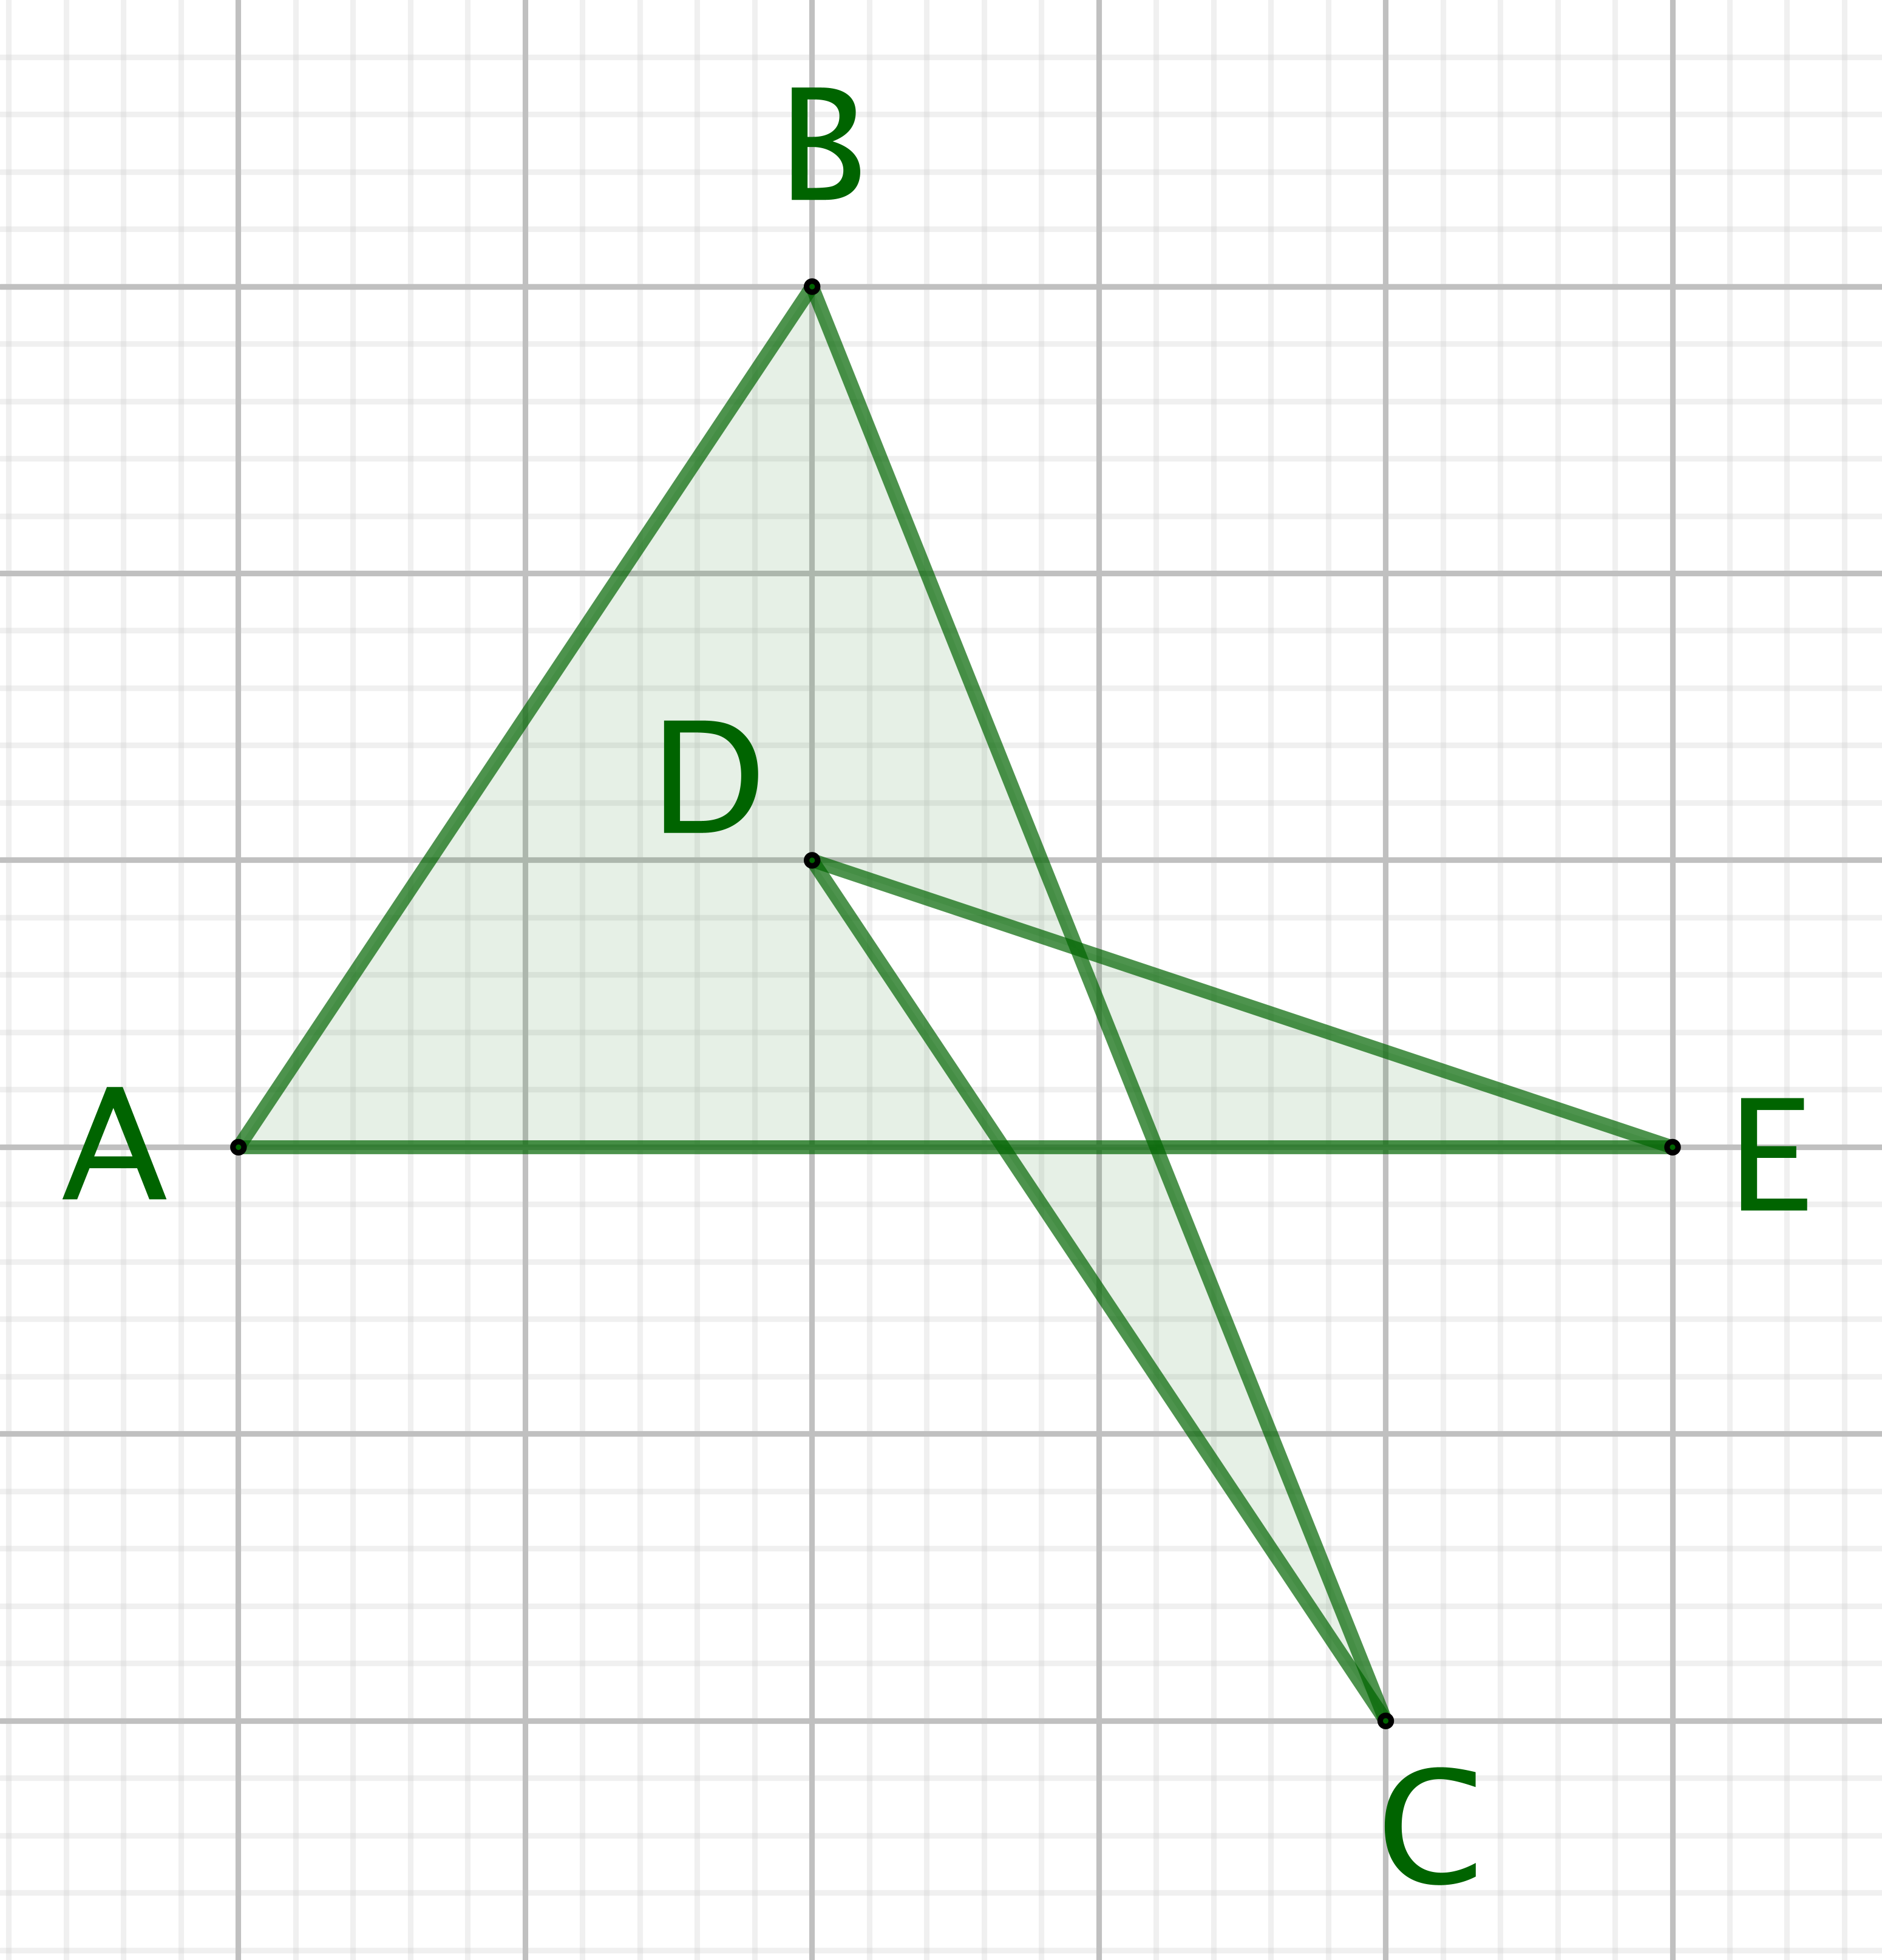
\includegraphics[scale=.4]{content/polygon/sufficient-cond/why.png}
    \end{center}
    
    \foreach \i in {3,1,4,2,5} {
    	\begin{center}
            \includegraphics[scale=.4]{content/polygon/sufficient-cond/why-step-\i.png}
        \end{center}
	}
\end{multicols}


Avant de formaliser ce qui précède, il faut noter que la notion d'aire algébrique est à manier avec prudence lorsqu'on la découvre. 
Si c'est votre cas, que pensez-vous de l'aire algébrique du quadrilatère croisé $ABCD$ ci-dessous qui est un antiparallélogramme très particulier? Réponse en note de bas de page.%
\footnote{
    La réponse est $0$. Comme nous verrons que le choix de $\Omega$ est libre, il suffit de faire les calculs avec $\Omega$ l'intersection des segments $[AD]$ et $[BC]$.
    On peut tout de même donner du sens à ceci. Voici comment. 
    Plongeons-nous dans l'espace. 
    Imaginons une toile rectangulaire rouge sur le dessus, et verte en dessous.
    Tournons de \qty{180}{\degree} verticalement l'un des côtés du rectangle.
    En supposant que la toile soit parfaitement tendue, nous obtenons, vue de dessus, un antiparallélogramme dont l'un des triangles est vert, et l'autre rouge.
    De façon savante, les deux faces ont deux orientations différentes. Nous reparlerons de cette notion par la suite.  
}

\begin{center}
    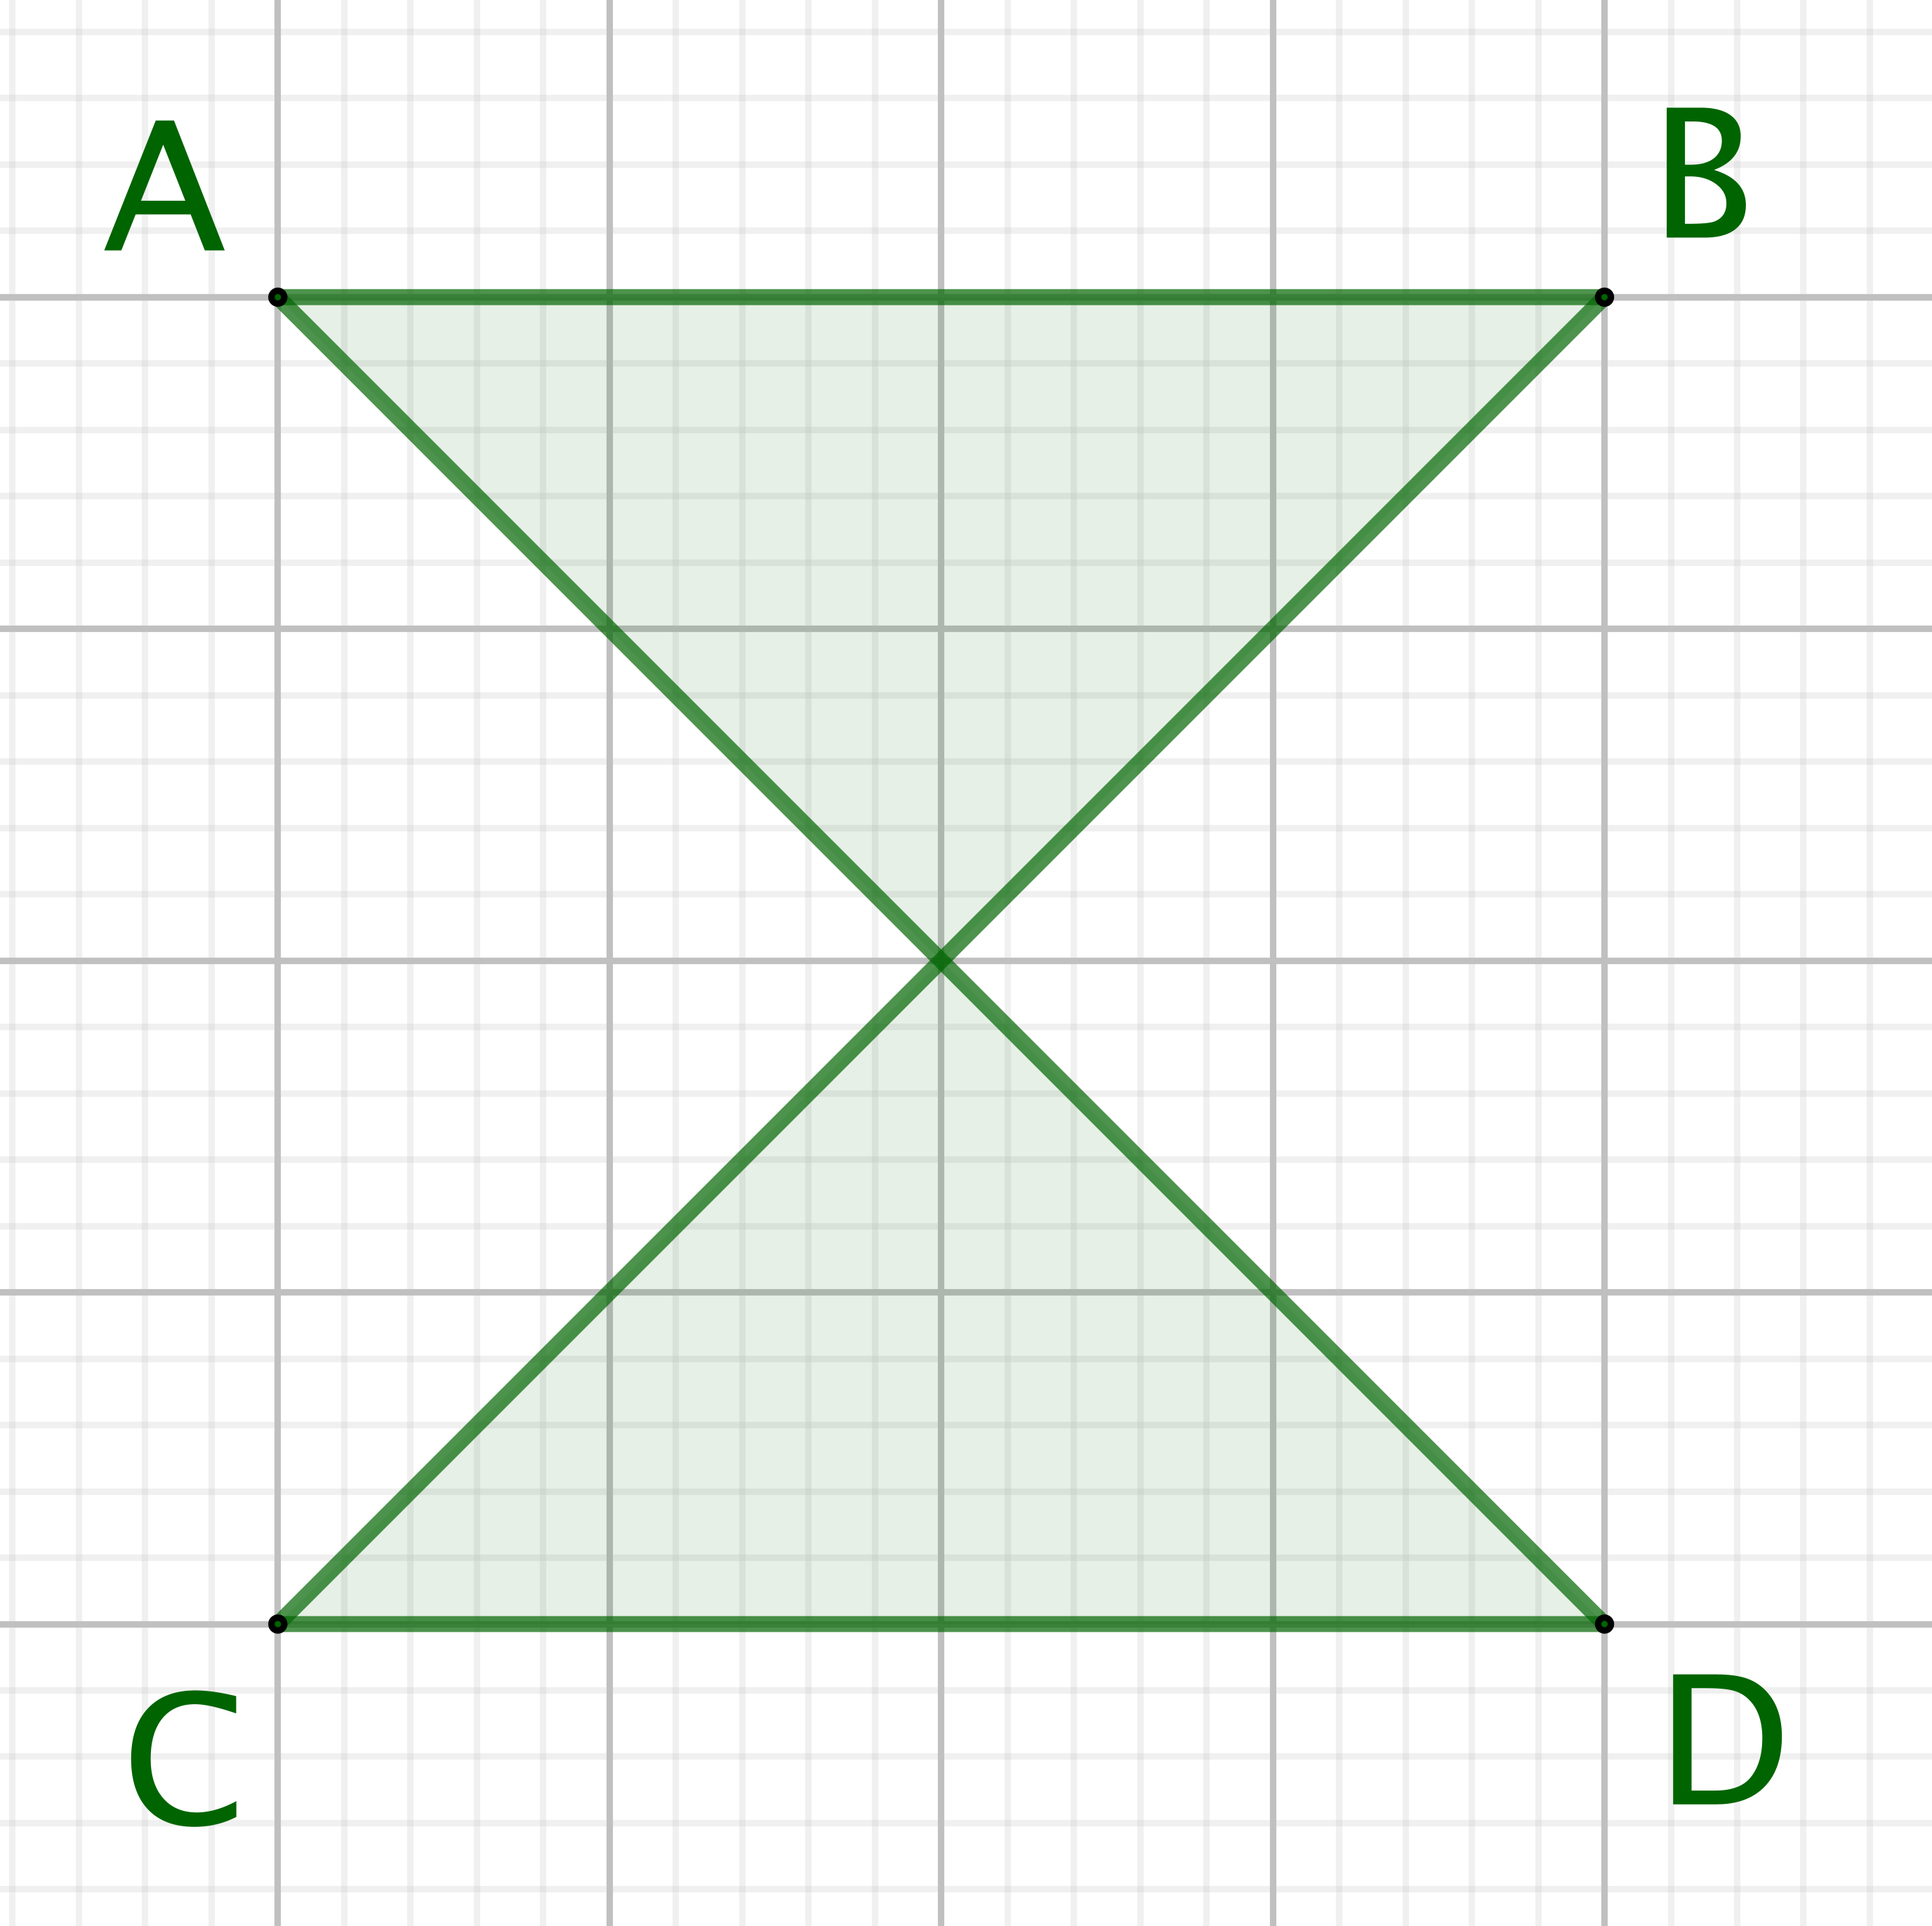
\includegraphics[scale=.4]{content/polygon/sufficient-cond/anti-para.png}
\end{center}


% ----------------------- %


\begin{defi} \label{garea-pt-ct}
    Pour toute \nline\  $\setproba{L} = A_1 A_2 \cdots A_n$, on définit $\big( A^{\,\prime}_i \big)_{i \in \ZZ}$ comme étant $n$-périodique, et vérifiant $A^{\,\prime}_{i} = A_i$ sur $\ZintervalC{1}{n}$.
\end{defi}


% ----------------------- %


\newpage

\begin{fact} \label{garea-pt-ct}
    Soit $\setproba{L} = A_1 A_2 \cdots A_n$ une \nline.
    La fonction qui à un point $\Omega$ du plan associe 
    $\mu_1^n (\Omega ;\setproba{L}) = \dsum_{i=1}^{n} \det \big( \vect{\Omega A^{\,\prime}_i} , \vect{\Omega A^{\,\prime}_{i+1}} \big)$ est indépendante du point $\Omega$.
    Dans la suite, cette quantité indépendante de $\Omega$ sera notée $\mu_1^n (\setproba{L})$.
\end{fact}


\begin{proof}
    Soit $M$ un autre point du plan.

    \begin{stepcalc}[style=ar*]
        \mu_1^n (\Omega ;\setproba{L})
    \explnext{}
        \dsum_{i=1}^{n} \det \big( \vect{\Omega A^{\,\prime}_i} , \vect{\Omega A^{\,\prime}_{i+1}} \big)
    \explnext*{Cette bonne vieille relation de Chasles.}{}
        \dsum_{i=1}^{n} \det \big( \vect{\Omega M} + \vect{M A^{\,\prime}_i} , \vect{\Omega M} + \vect{M A^{\,\prime}_{i+1}} \big)
    \explnext{}
        \dsum_{i=1}^{n} \Big[
            \det \big( \vect{\Omega M} , \vect{\Omega M} \big)
            +
            \det \big( \vect{\Omega M} , \vect{M A^{\,\prime}_{i+1}} \big)
            +
            \det \big( \vect{M A^{\,\prime}_i} , \vect{\Omega M} \big)
            +
            \det \big( \vect{M A^{\,\prime}_i} , \vect{M A^{\,\prime}_{i+1}} \big)
        \Big]
    \explnext{}
        \dsum_{i=1}^{n} \det \big( \vect{\Omega M} , \vect{M A^{\,\prime}_{i+1}} \big)
        +
        \dsum_{i=1}^{n} \det \big( \vect{M A^{\,\prime}_i} , \vect{\Omega M} \big)
        +
        \mu_1^n (M ; \setproba{L})
    \explnext{}
        \mu_1^n (M ; \setproba{L})
        +
        \dsum_{i=2}^{n+1} \det \big( \vect{\Omega M} , \vect{M A^{\,\prime}_{i}} \big)
        -
        \dsum_{i=1}^{n} \det \big( \vect{\Omega M} , \vect{M A^{\,\prime}_i} \big)
    \explnext{}
        \mu_1^n (M ; \setproba{L})
        +
        \det \big( \vect{\Omega M} , \vect{M A^{\,\prime}_{n+1}} \big)
        -
        \det \big( \vect{\Omega M} , \vect{M A^{\,\prime}_1} \big)
    \explnext*{$A^{\,\prime}_{n+1} = A^{\,\prime}_1$}{}
        \mu_1^n (M ; \setproba{L})
    \end{stepcalc}
    
    \null\vspace{-3.5ex}
\end{proof}
    
    
% ----------------------- %


\begin{fact} \label{nline-shift-inva}
    Soit $\setproba{L} = A_1 A_2 \cdots A_n$ une \nline.
    Pour $k \in \ZintervalC{1}{n}$, 
    la \nline\ $\setproba{L}_j = B_1 B_2 \cdots B_n$, où $B_i = A^{\,\prime}_{k+i-1}$,
    vérifie
    $\mu_1^n (\setproba{L}) = \mu_1^n (\setproba{L}_k)$.
    Dans la suite, cette quantité commune sera notée $\mu (\setproba{L})$.
\end{fact}


\begin{proof}
    Il suffit de s'adonner à un petit jeu sur les indices de sommation.
\end{proof}
    
    
% ----------------------- %


\begin{fact} \label{nline-rota-inva}
    Soit 
    $\setproba{L} = A_1 A_2 \cdots A_n$ une \nline. 
    La \nline\ $\setproba{L}^{\mathrm{op}} = B_1 B_2 \cdots B_n$, où $B_i =  A_{n + 1 - i}$,
    vérifie
    $\mu(\setproba{L}^{\mathrm{op}}) = {} - \mu(\setproba{L})$.
\end{fact}


\begin{proof}
    Soit $\Omega$ un point quelconque du plan.

    \begin{stepcalc}[style=ar*]
        \mu(\setproba{L}^{\mathrm{op}})
    \explnext{}
        \dsum_{i=1}^{n} \det \big( \vect{\Omega B^{\,\prime}_i} , \vect{\Omega B^{\,\prime}_{i+1}} \big)
    \explnext{}
        \dsum_{i=1}^{n} \det \big( \vect{\Omega A^{\,\prime}_{n + 1 - i}} , \vect{\Omega A^{\,\prime}_{n - i}} \big)
    \explnext{}
        \dsum_{j=0}^{n-1} \det \big( \vect{\Omega A^{\,\prime}_{j + 1}} , \vect{\Omega A^{\,\prime}_j} \big)
    \explnext*{$A^{\,\prime}_0 = A^{\,\prime}_n$ et $A^{\,\prime}_1 = A^{\,\prime}_{n+1}$}{}
        \dsum_{j=1}^{n} \det \big( \vect{\Omega A^{\,\prime}_{j + 1}} , \vect{\Omega A^{\,\prime}_j} \big)
    \explnext{}
        {} - \dsum_{j=1}^{n} \det \big( \vect{\Omega A^{\,\prime}_j} ,  \vect{\Omega A^{\,\prime}_{j + 1}} \big)
    \explnext{}
        {} - \mu(\setproba{L})
    \end{stepcalc}
    
    \null\vspace{-3.5ex}
\end{proof}
    
    
% ----------------------- %


\begin{fact}
    Soit 
    $\setproba{L} = A_1 A_2 \cdots A_n$ une \nline.
    La quantité $\frac12 \abs{\mu(\setproba{L})}$ ne dépend ni du sens de parcours de $\setproba{L}$, ni du point de départ choisi.%
    \footnote{
        Le lecteur pardonnera les abus de langage utilisés.
    }
    Elle sera notée $\garea{\setproba{L}}$, et nommée \og \emph{aire généralisée} \fg\ de la \nline\ $\setproba{L}$.
\end{fact}


\begin{proof}
    C'est une conséquence directe des faits \ref{nline-shift-inva} et \ref{nline-rota-inva}.
\end{proof}
    
    
% ----------------------- %


Pour notre démonstration finale, nous aurons besoin de savoir que $\garea{\setproba{P}} = \area{\setproba{P}}$ pour tout \ngone\ $\setproba{P}$.%
\footnote{
	Nous obtenons ainsi la généralisation de l'aire géométrique usuelle au cas des polygones croisés.
}
Ceci est évident dans le cas convexe, car il suffit de choisir l'isobarycentre $G$ de $A_1$, $A_2$, ..., $A_n$ pour le calcul de $\garea{\setproba{P}}$: en effet, avec ce choix, tous les déterminants $\det \big( \vect{G A^{\,\prime}_i} , \vect{G A^{\,\prime}_{i+1}} \big)$ ont le même signe.
Dans le cas non-convexe, les choses se compliquent a priori, car nous ne maîtrisons plus les signes des déterminants. Heureusement nous avons le résultat fort suivant qui est un pas important pour atteindre notre but.


\begin{fact} \label{route-direction}
    Soit un \ngone\ $\setproba{P}$.
    On suppose la \nline\ $\setproba{L} = A_1 A_2 \cdots A_n$ associée à $\setproba{P}$ telle que les points $A_1$, $A_2$, ..., $A_n$ soient parcourus dans le sens trigonométrique, ou anti-horaire. Une telle \nline\ sera dite \og \emph{positive} \fg.%
    \footnote{
    	Bien noté que cette notion ne peut exister lorsqu'on considère un polygone croisé. De façon cachée, nous utilisons le célèbre théorème de Jordan, dans sa forme polygonale. 
    }
    Sous cette hypothèse, nous avons $\mu(\setproba{L}) \geq 0$.
\end{fact}


\begin{proof}
	Le théorème de triangulation affirme que tout \ngone\ est triangulable comme dans l'exemple très basique suivant qui laisse envisager une démonstration par récurrence en retirant l'un des triangles ayant deux côtés correspondant à deux côtés consécutifs du \ngone\ (pour peu qu'un tel triangle existe toujours).

    
    \begin{multicols}{3}
        \small\itshape
        \begin{center}
            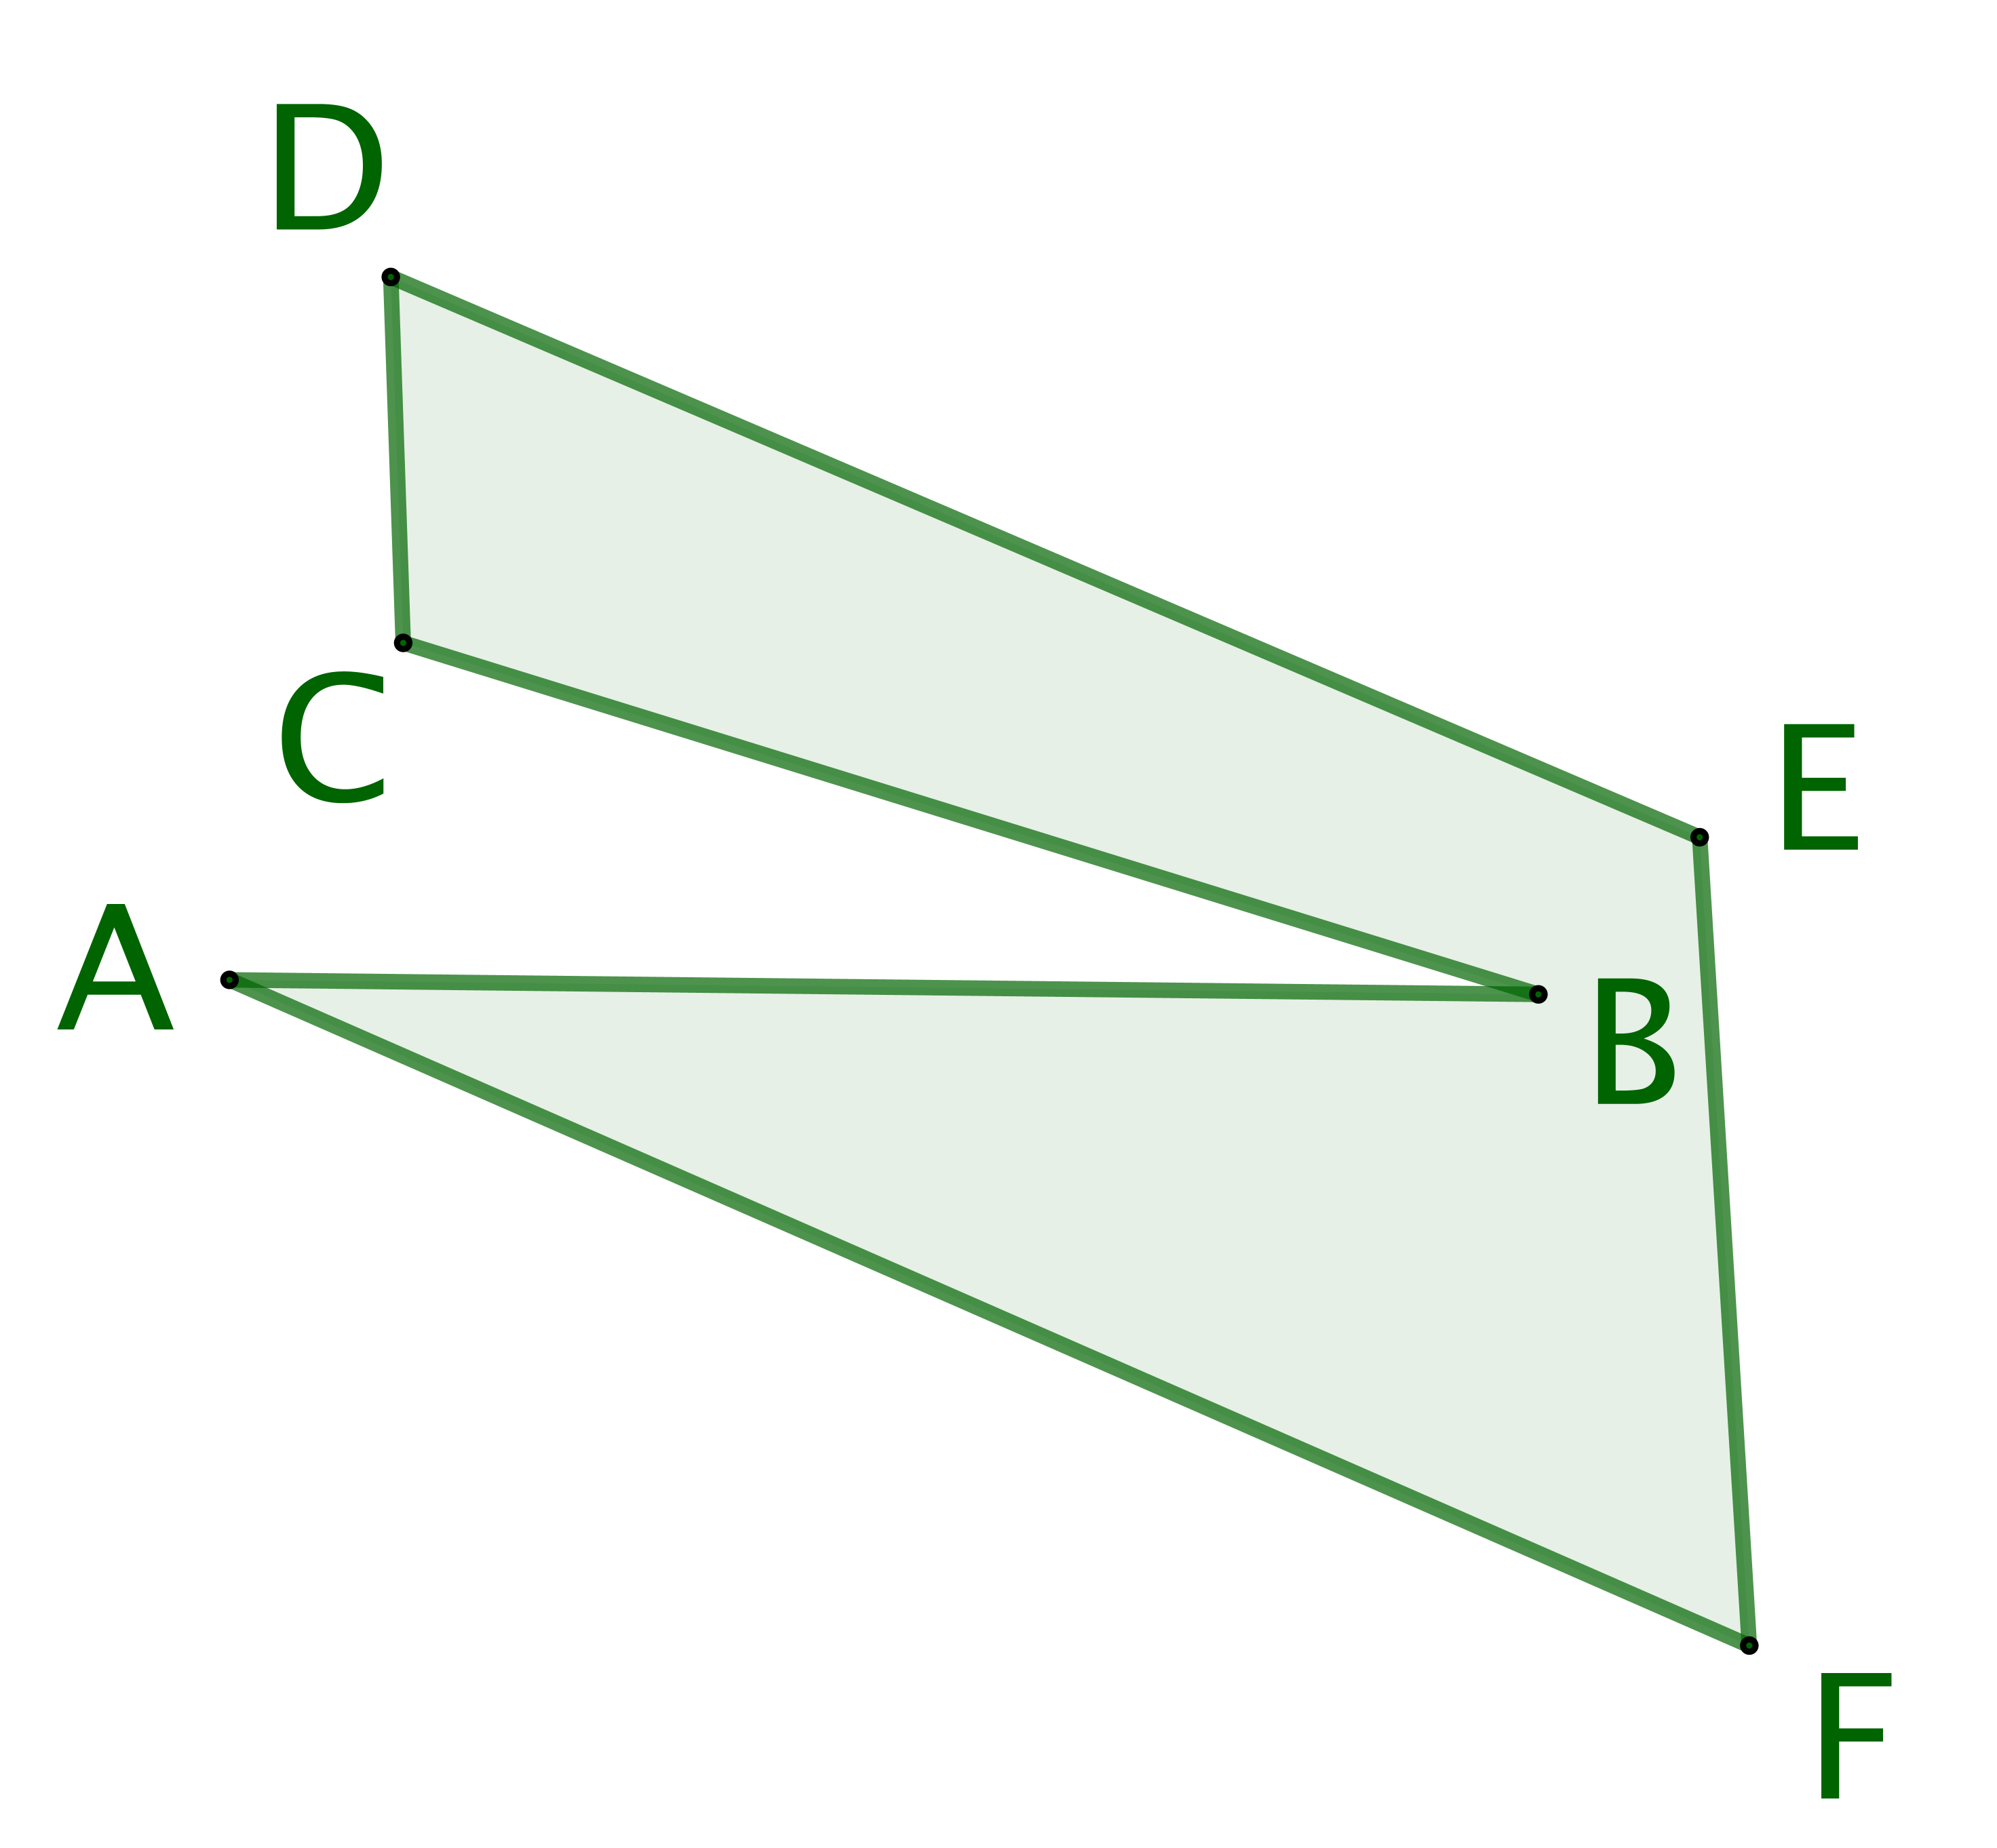
\includegraphics[scale=.4]{content/polygon/sufficient-cond/triangulation-1.png}
        
            \smallskip
            Un \ngone\ nu.
        \end{center}

    
        \begin{center}
            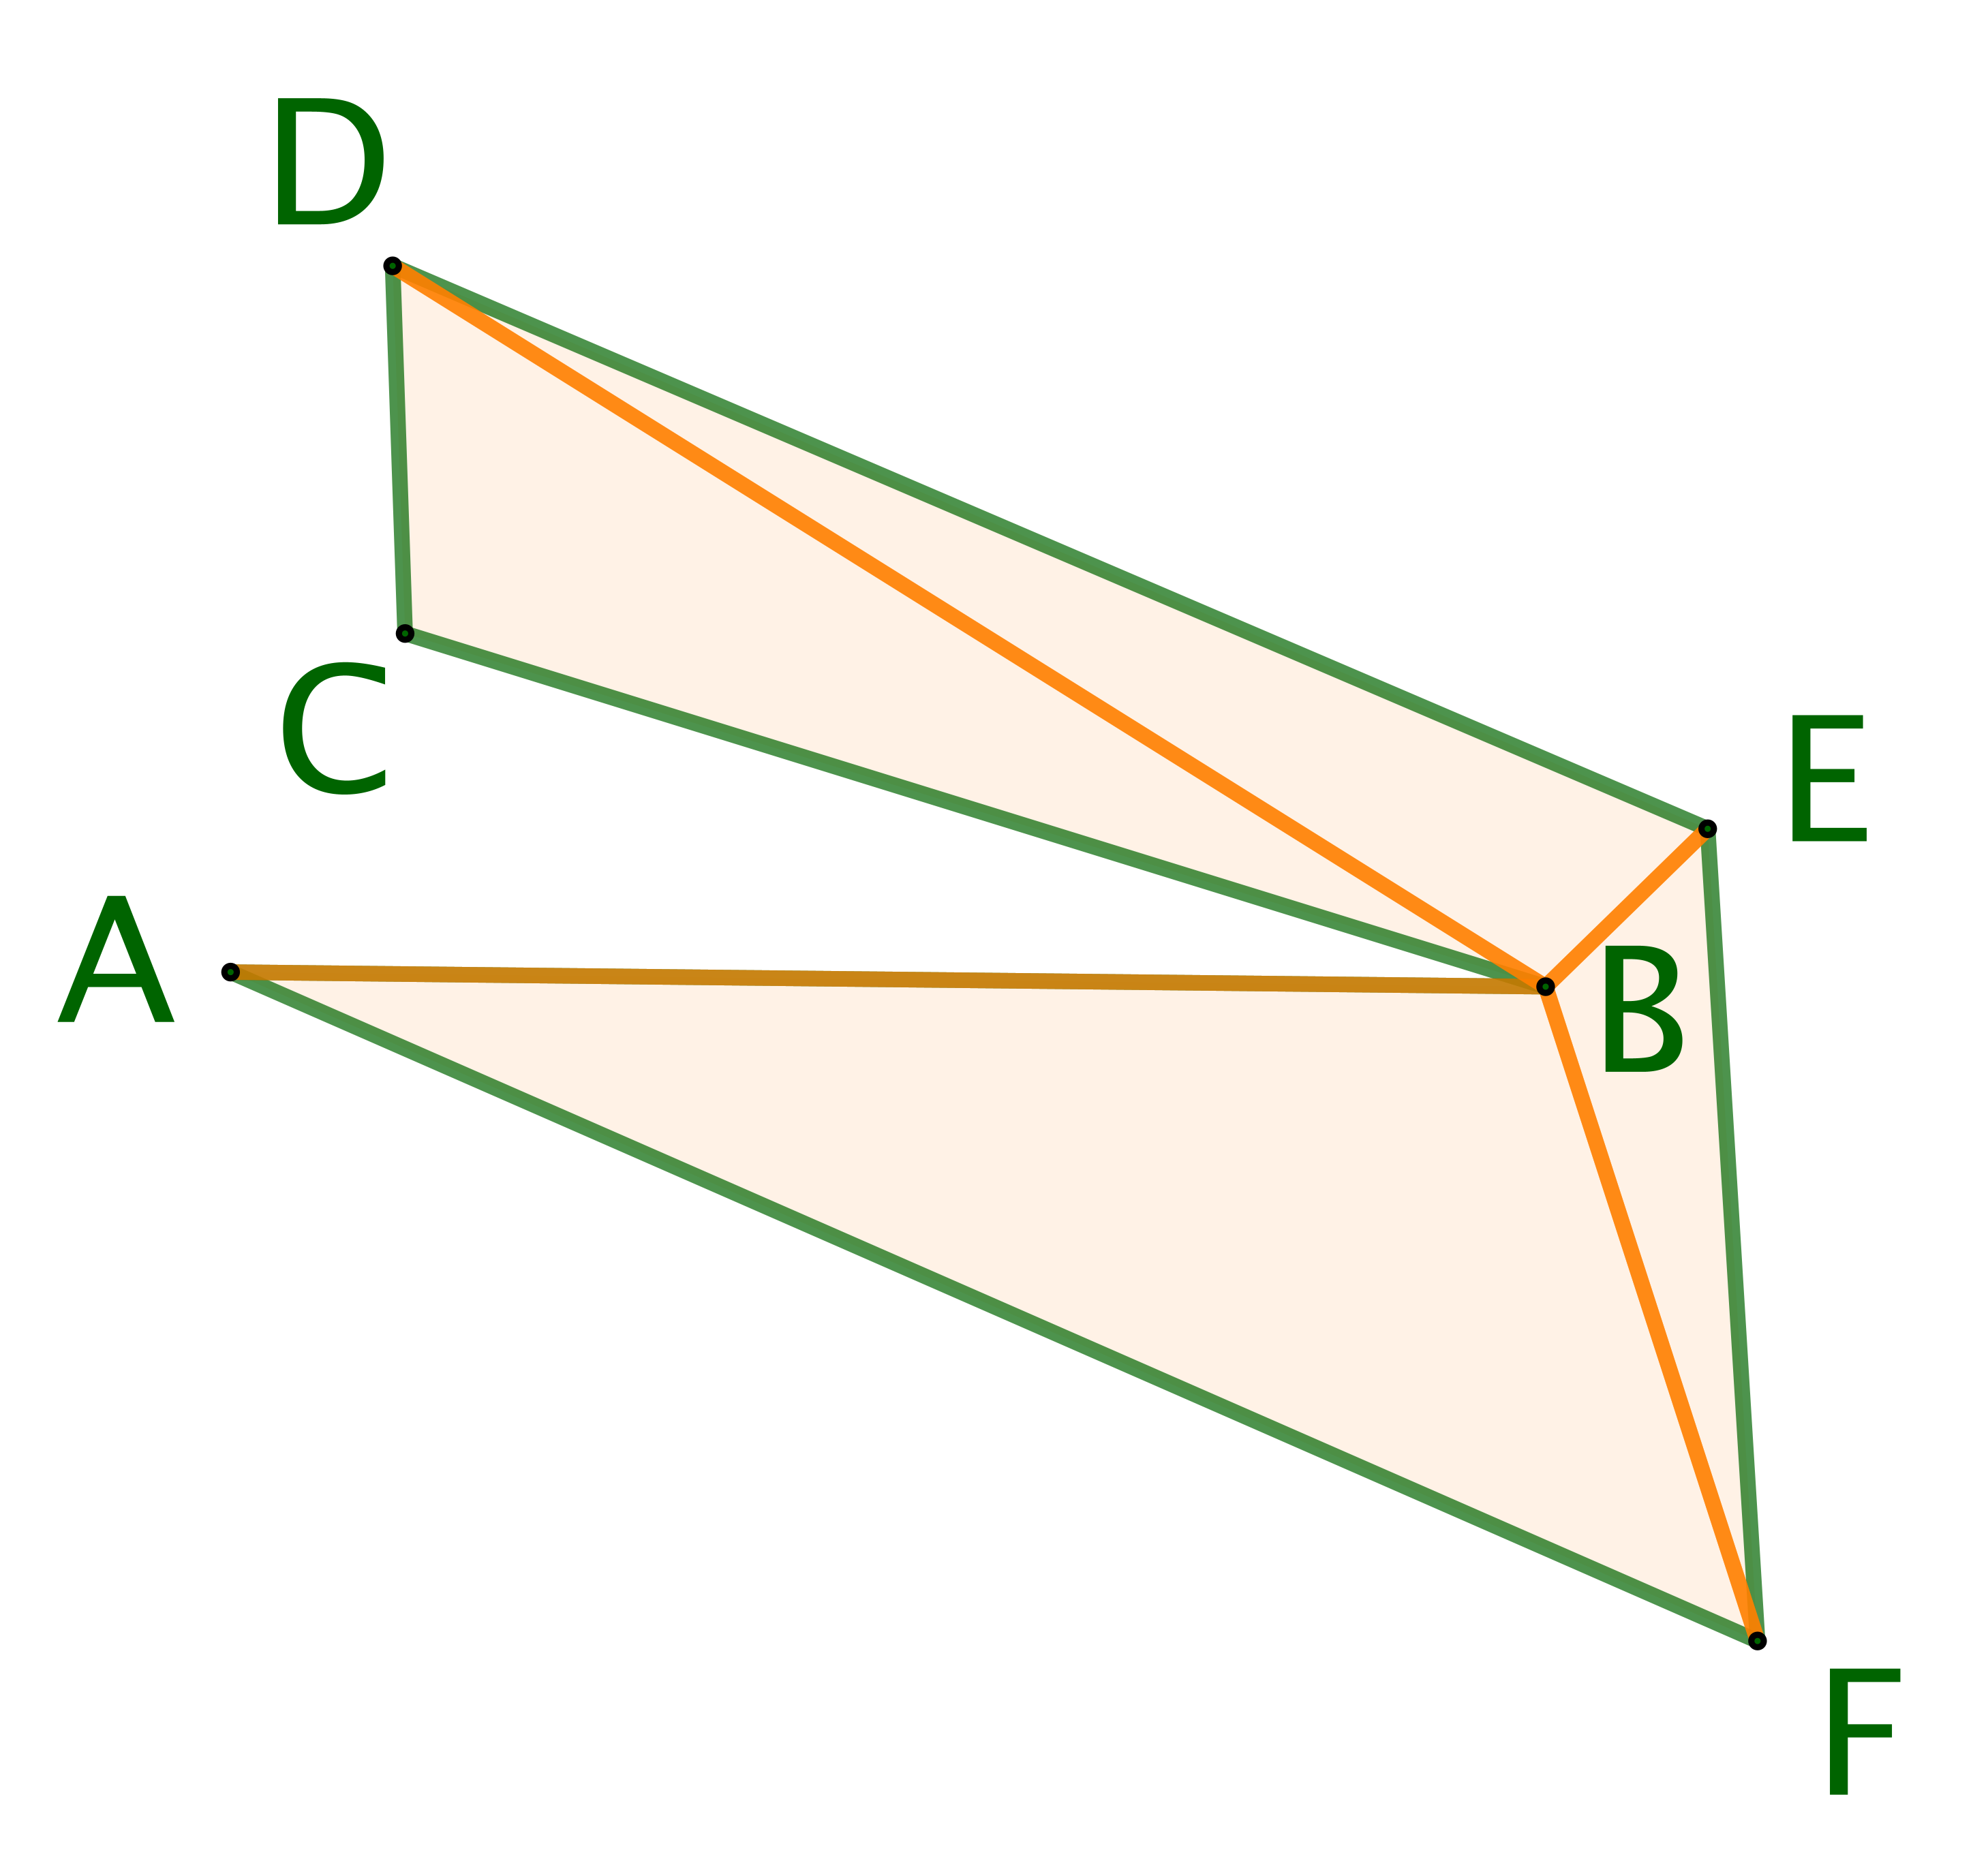
\includegraphics[scale=.4]{content/polygon/sufficient-cond/triangulation-2.png}
        
            \smallskip
            Le \ngone\ triangulé.
        \end{center}

    
        \begin{center}
            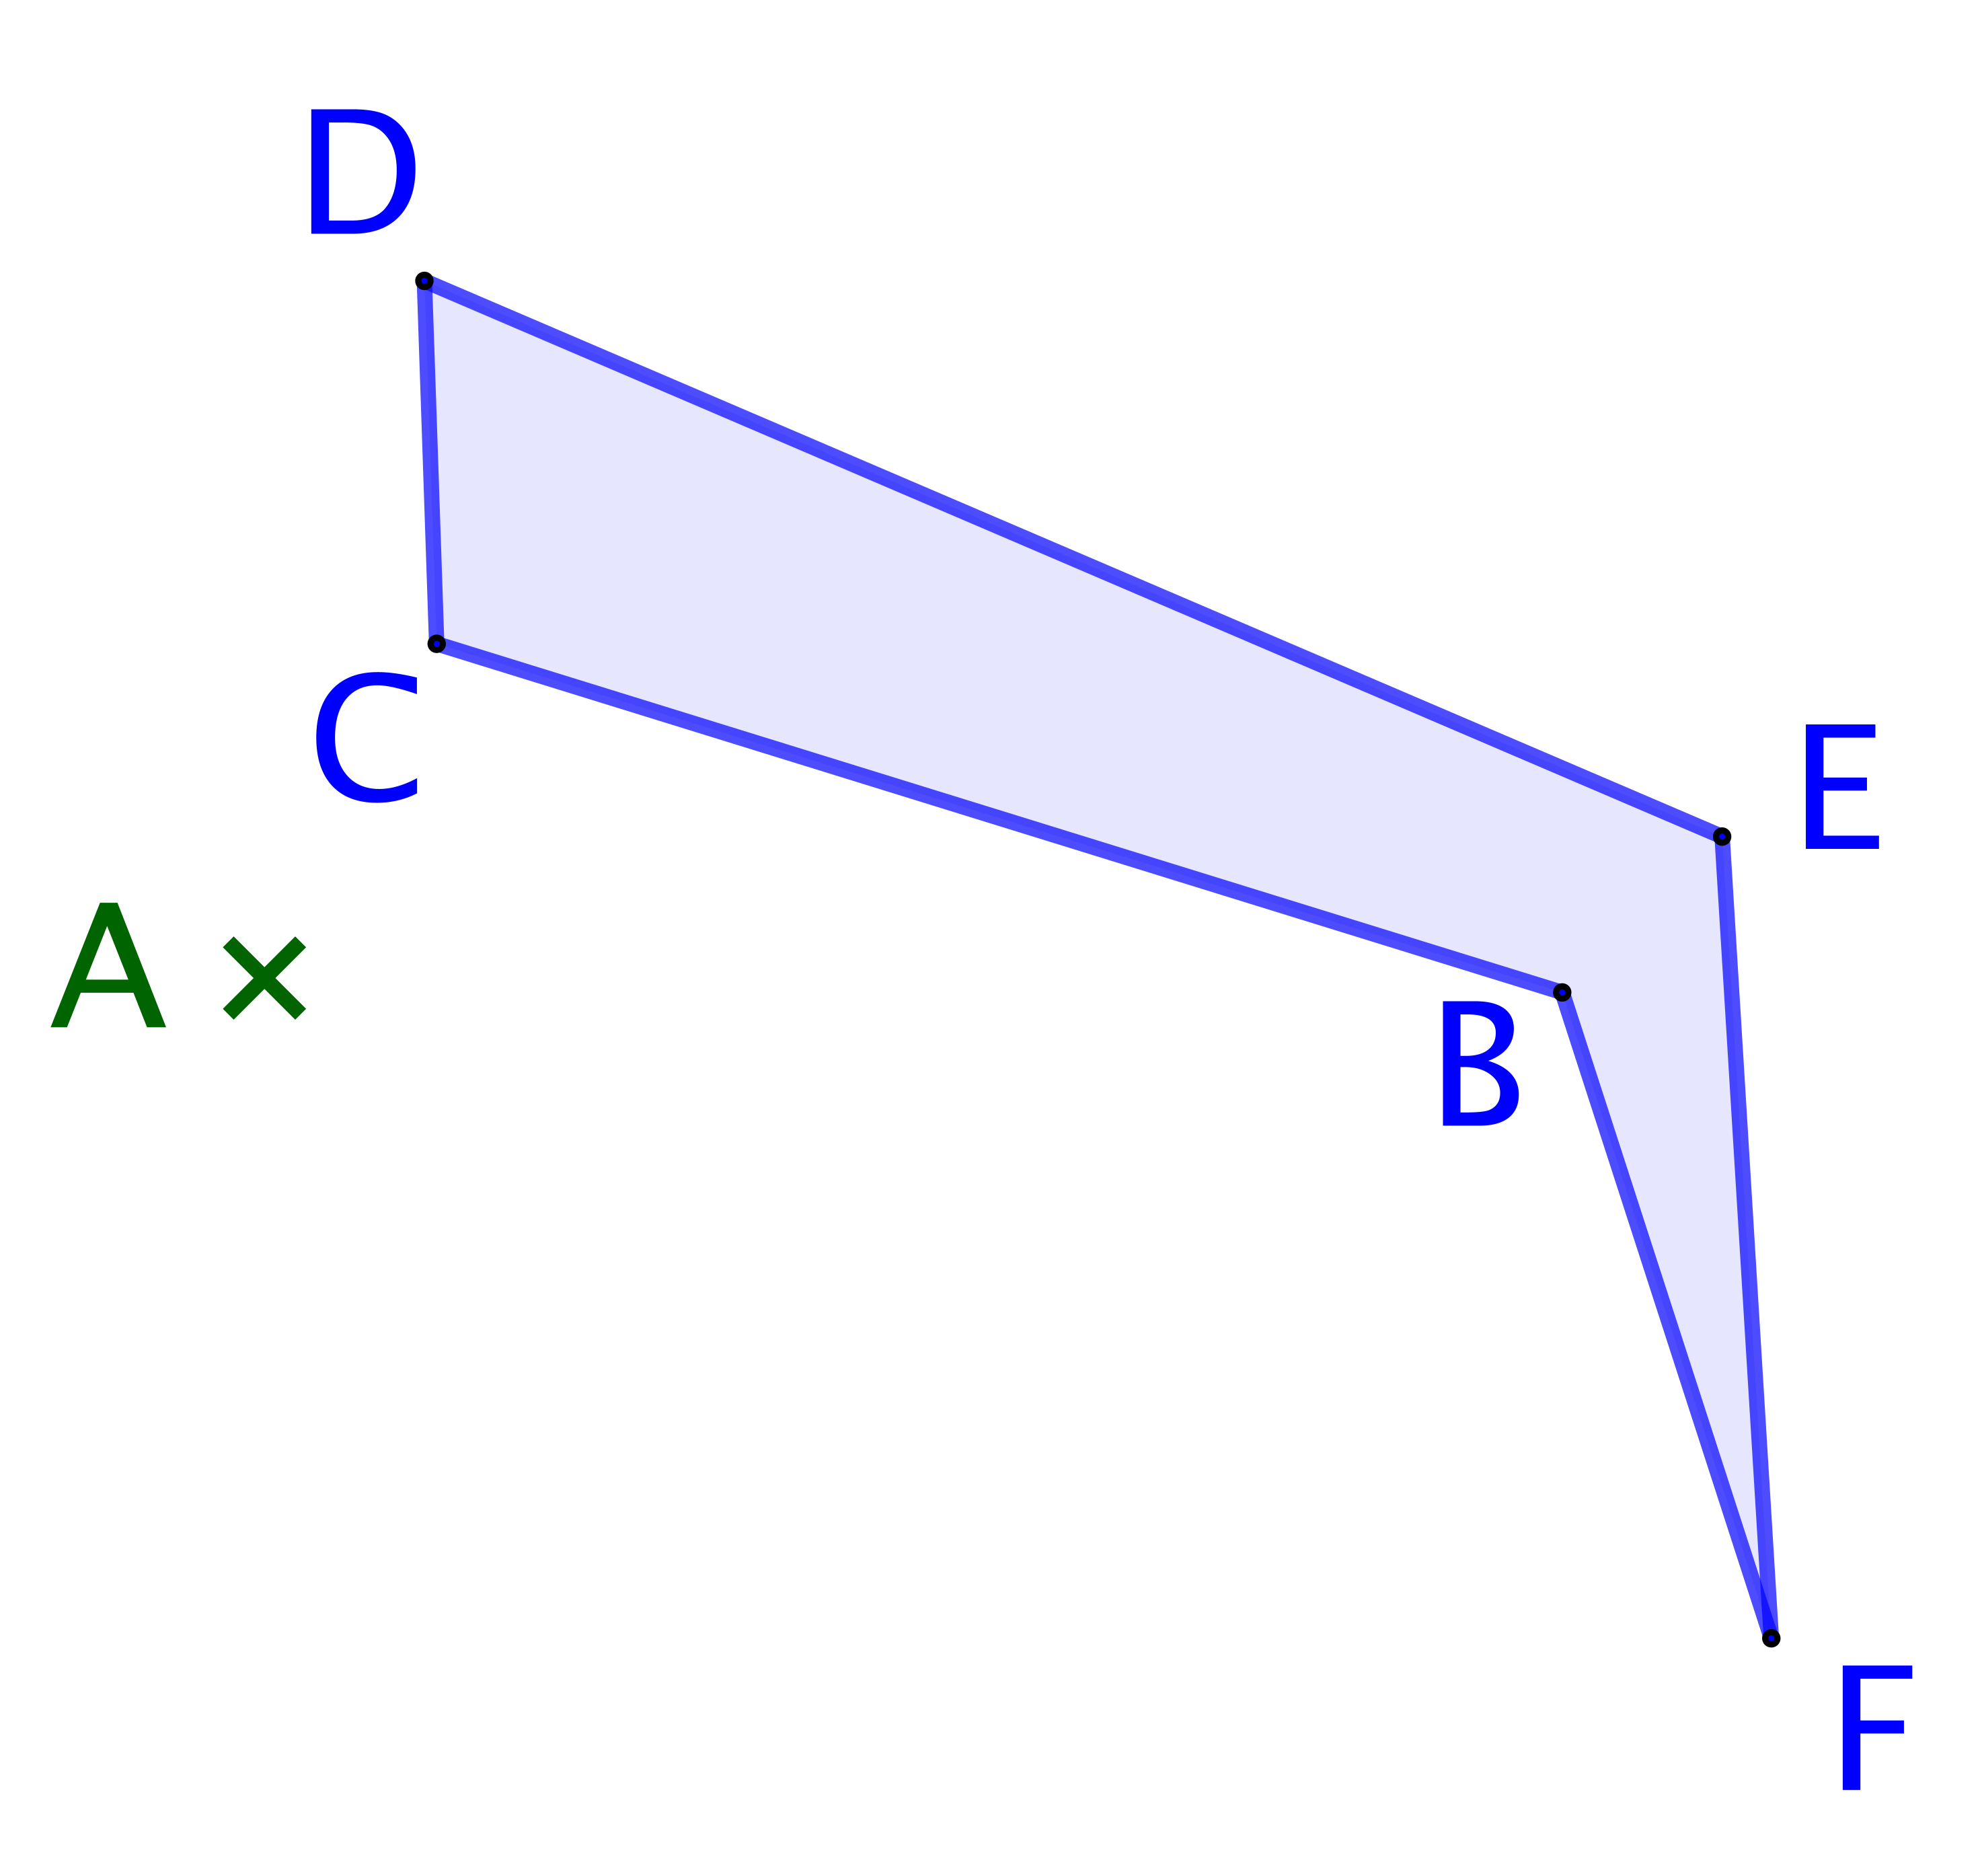
\includegraphics[scale=.4]{content/polygon/sufficient-cond/triangulation-3.png}
        
            \smallskip
            Le \ngone\ allégé.
        \end{center}
    \end{multicols}
    
    
    Le théorème de triangulation admet une forme forte donnant une décomposition contenant un triangle formé de deux côtés consécutifs du \ngone.%
    \footnote{
        En pratique, cette forme forte est peu utile, car elle aboutit à un algorithme de recherche trop lent.
    }
    Nous dirons qu'une telle décomposition est \og \emph{à l'écoute} \fg.
    Ce très mauvais jeu de mots fait référence à la notion sérieuse \og \emph{d'oreille} \fg\ pour un \ngone: une oreille est un triangle inclus dans le \ngone, et formé de deux côtés consécutifs du \ngone.
    L'exemple suivant donne un \ngone\ n'ayant que deux oreilles: ceci montre que l'existence d'une oreille ne va pas de soi.%
    \footnote{
        On démontre que tout \ngone\ admet au minimum deux oreilles.
    }


    \begin{multicols}{2}
        \small\itshape
    	\begin{center}
        	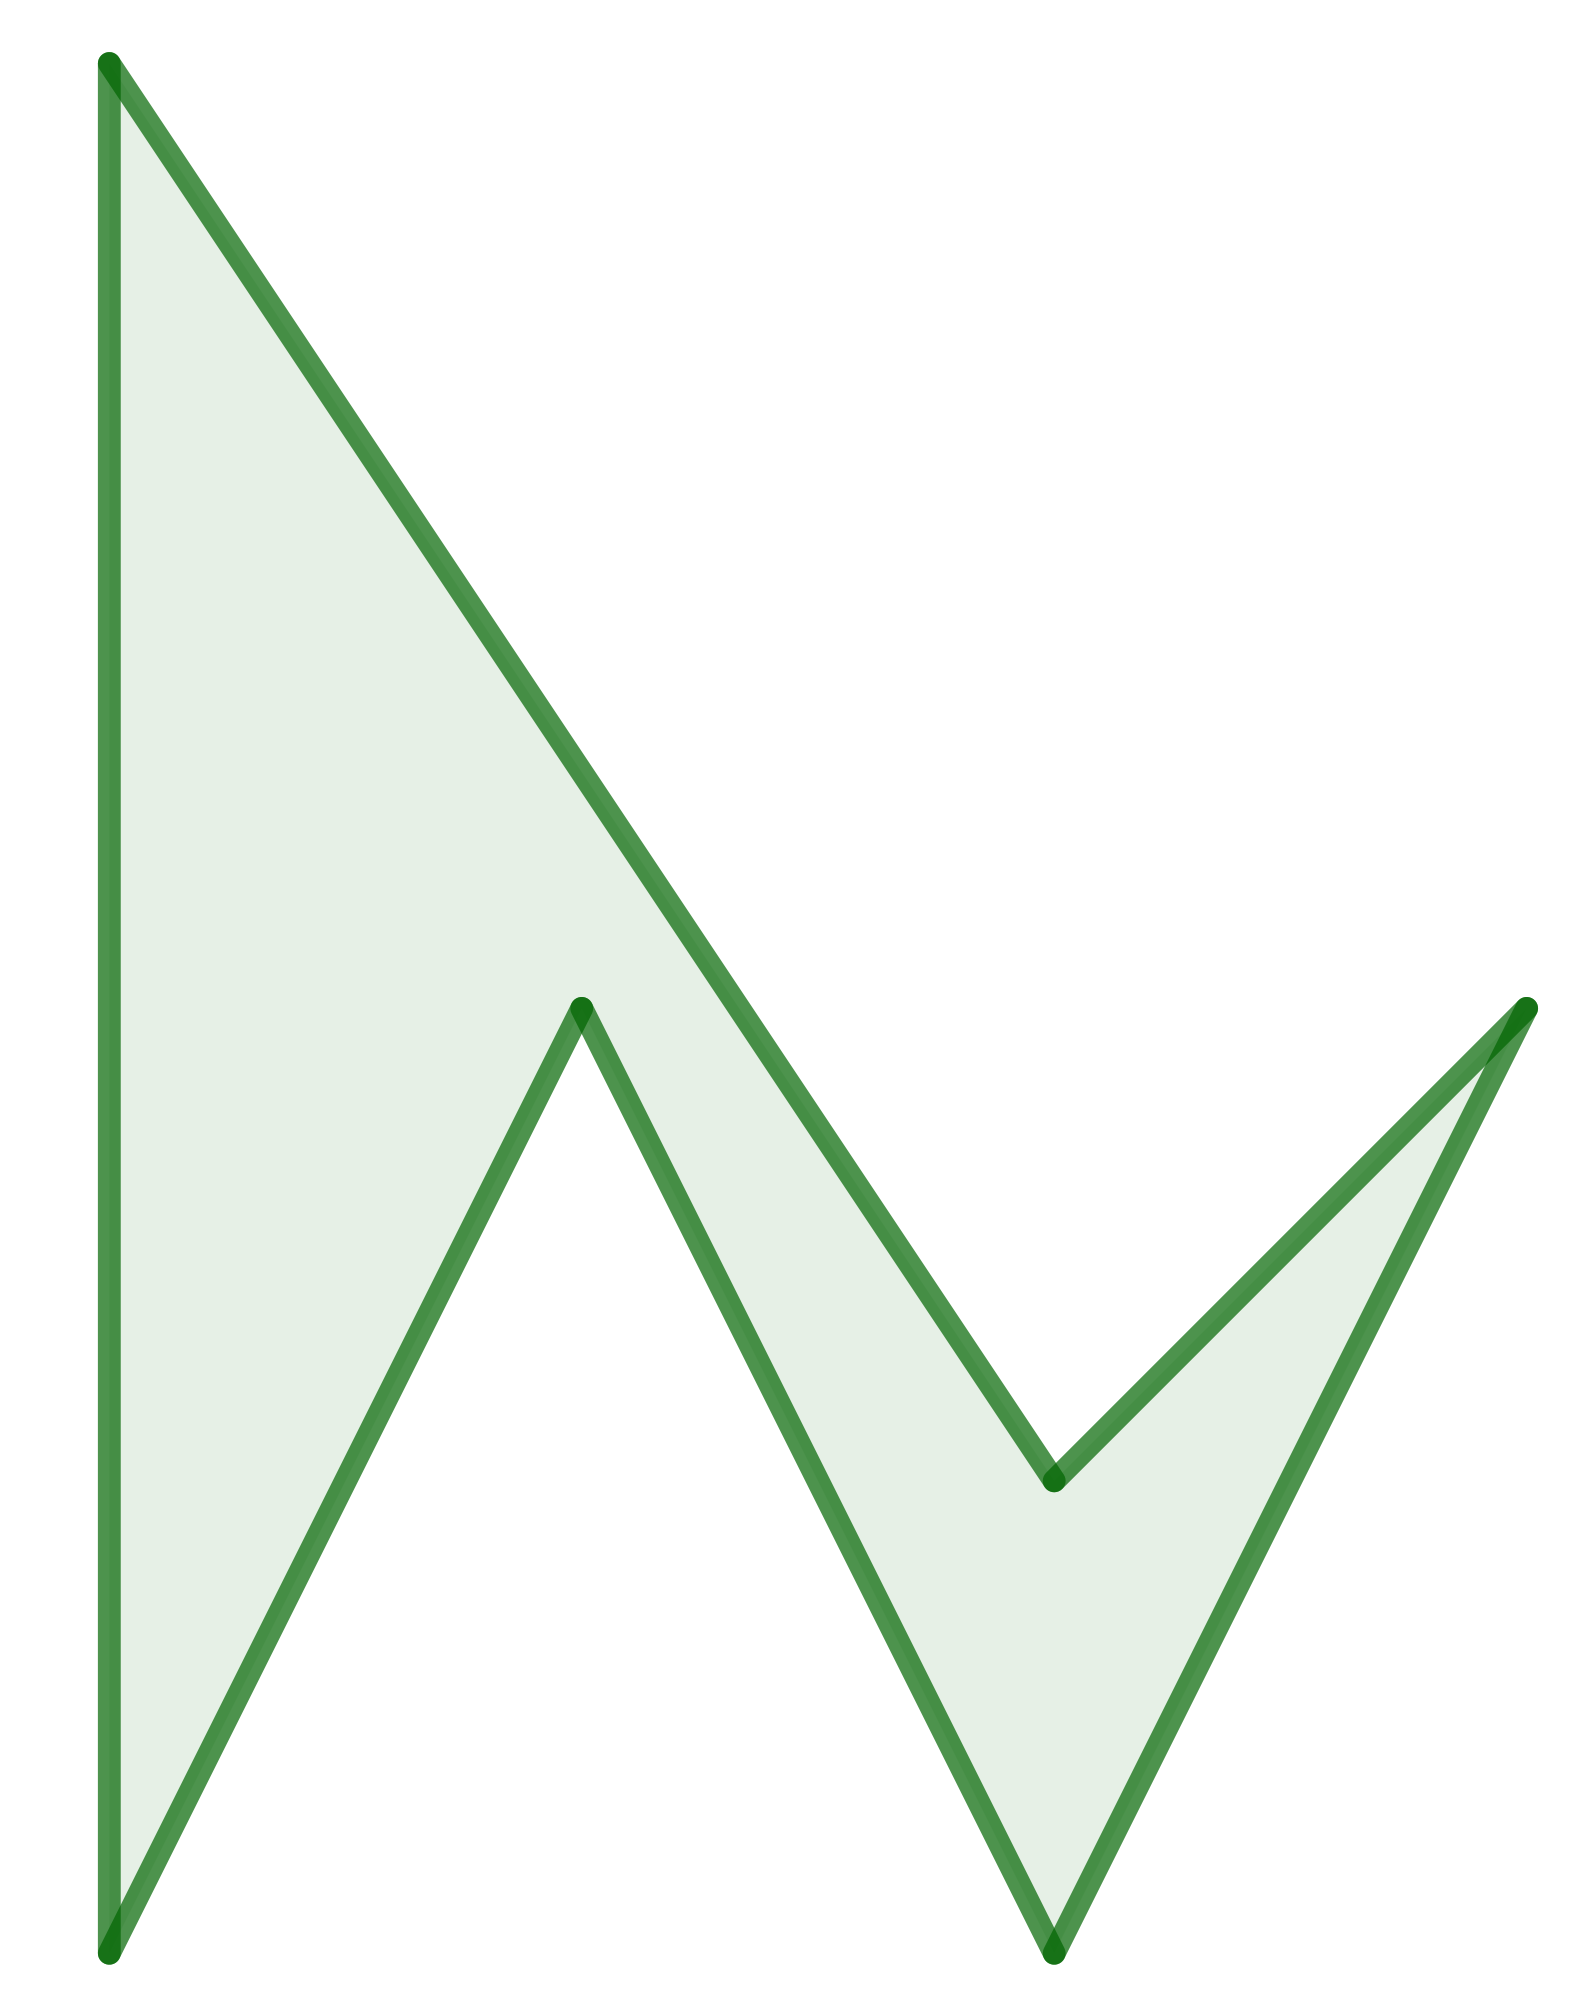
\includegraphics[scale=.4]{content/polygon/sufficient-cond/mini-ear-1.png}
        
        	\smallskip
       		Un \ngone\ basique.
    	\end{center}
	
    	\begin{center}
        	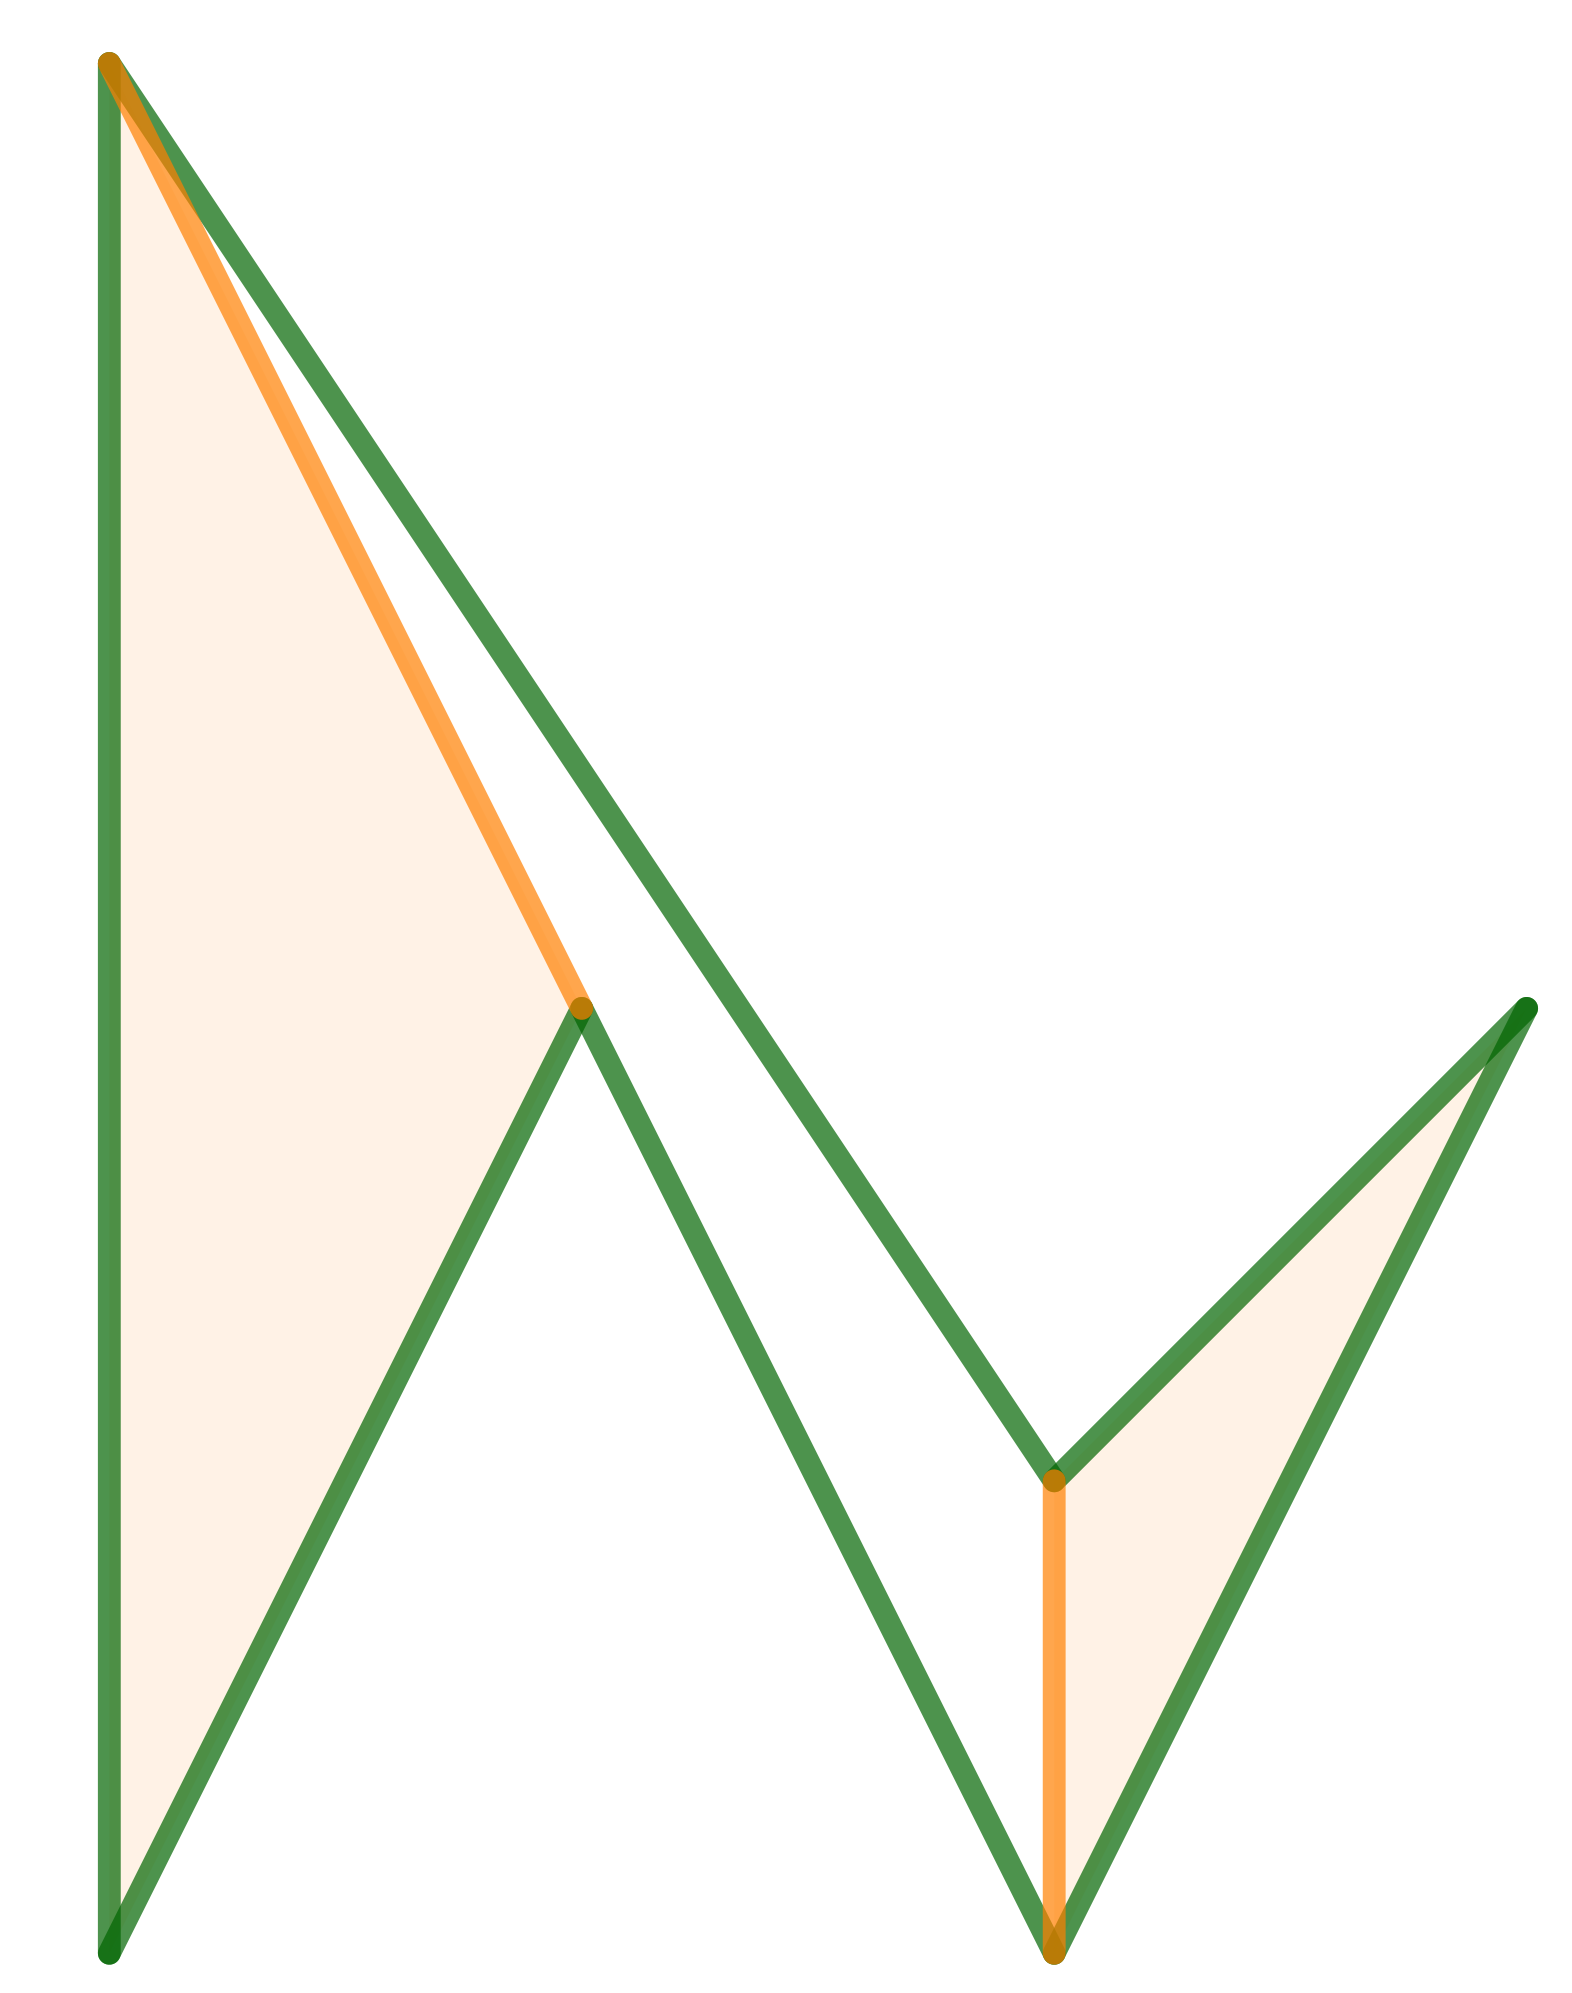
\includegraphics[scale=.4]{content/polygon/sufficient-cond/mini-ear-2.png}
        
        	\smallskip
       		Juste deux oreilles disponibles.
    	\end{center}
    \end{multicols}
    
    
	Nous allons raisonner par récurrence sur $n \in \NN_{\geq3}$.
	
	\begin{itemize}
		\item \textbf{Cas de base.} 
		Soit $ABC$ un triangle. Dire que les sommets $A$, $B$ et $C$ sont parcourus dans le sens trigonométrique, c'est savoir que $\mu(ABC) = \det \big( \vect{AB} , \vect{AC} \big) > 0$.


		\item \textbf{Hérédité.} 
		Soient un \ngone\ $\setproba{P}$, avec $n \in \NN_{>3}$, et $\setproba{L} = A_1 A_2 \cdots A_n$ une \nline\ positive qui lui est associée. On peut supposer que $A_{n-1} A_n A_1$ est une oreille du \ngone\ $\setproba{P}$.


	    \begin{multicols}{2}
    	    \small\itshape
    		\begin{center}
        	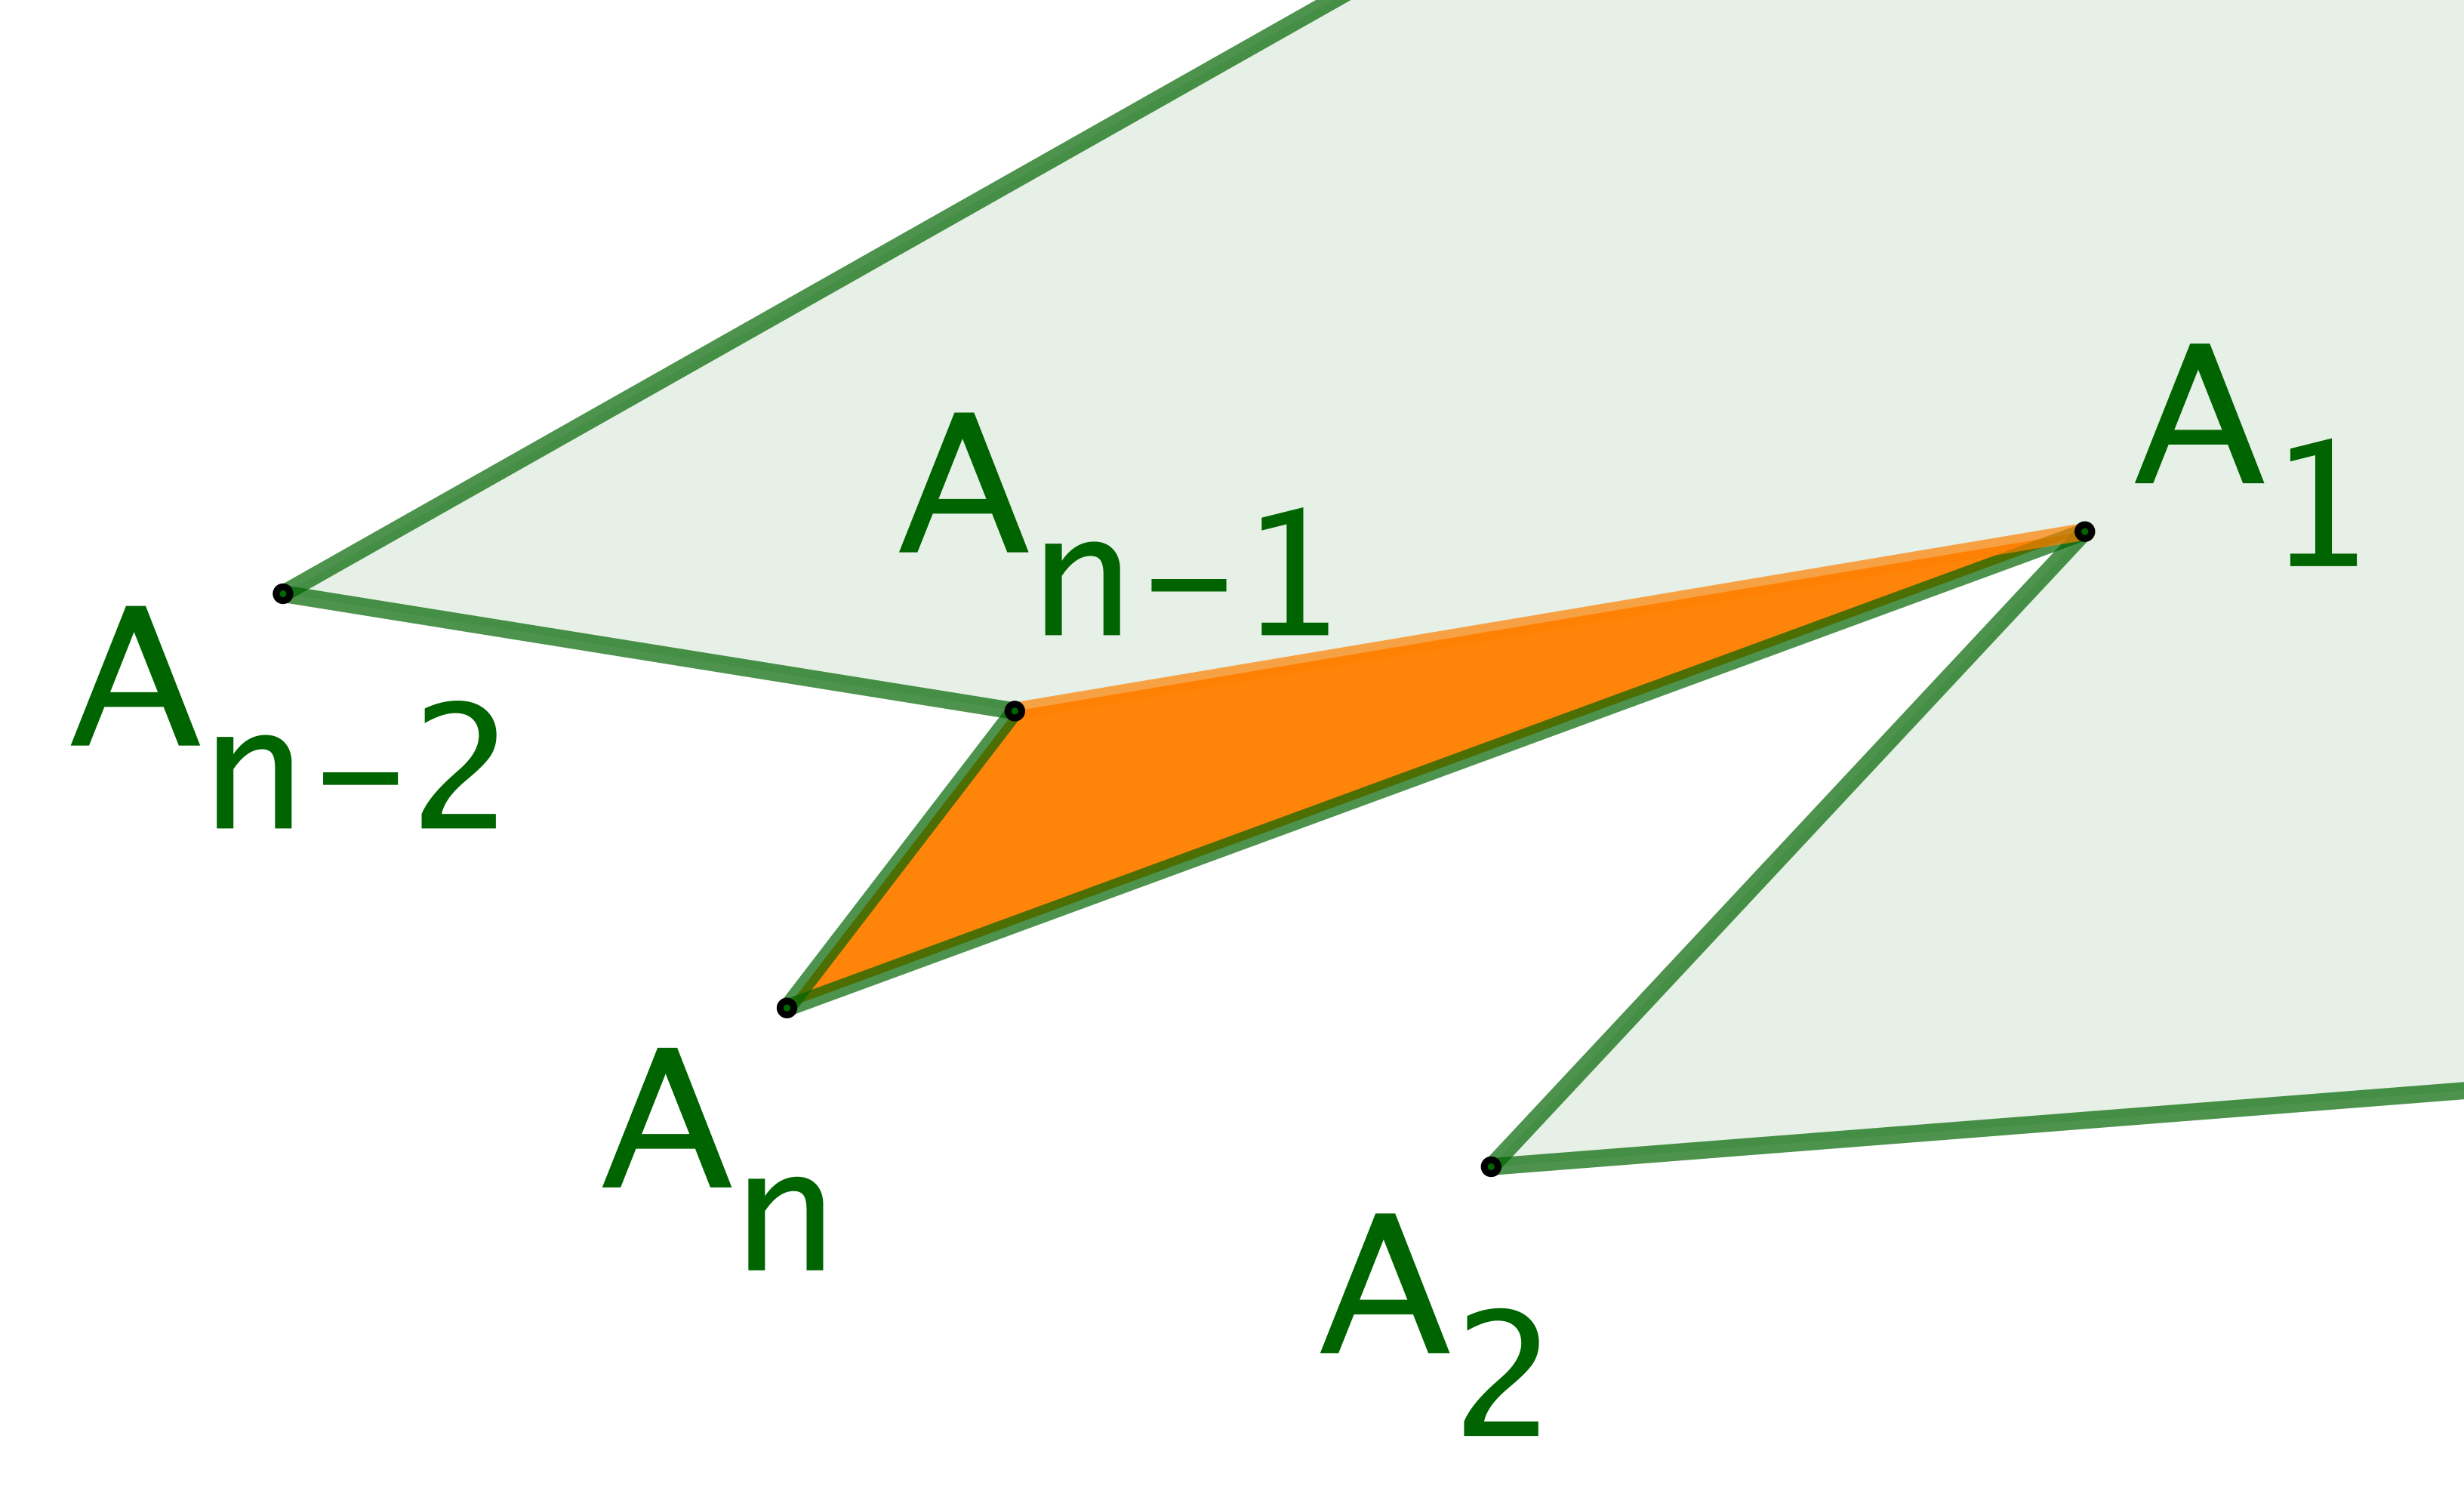
\includegraphics[scale=.4]{content/polygon/sufficient-cond/triangulation-proof-OK.png}
        
	        	\smallskip
    	   		$A_{n-1} A_n A_1$ est une oreille.
    	\end{center}
	
	    	\begin{center}
        	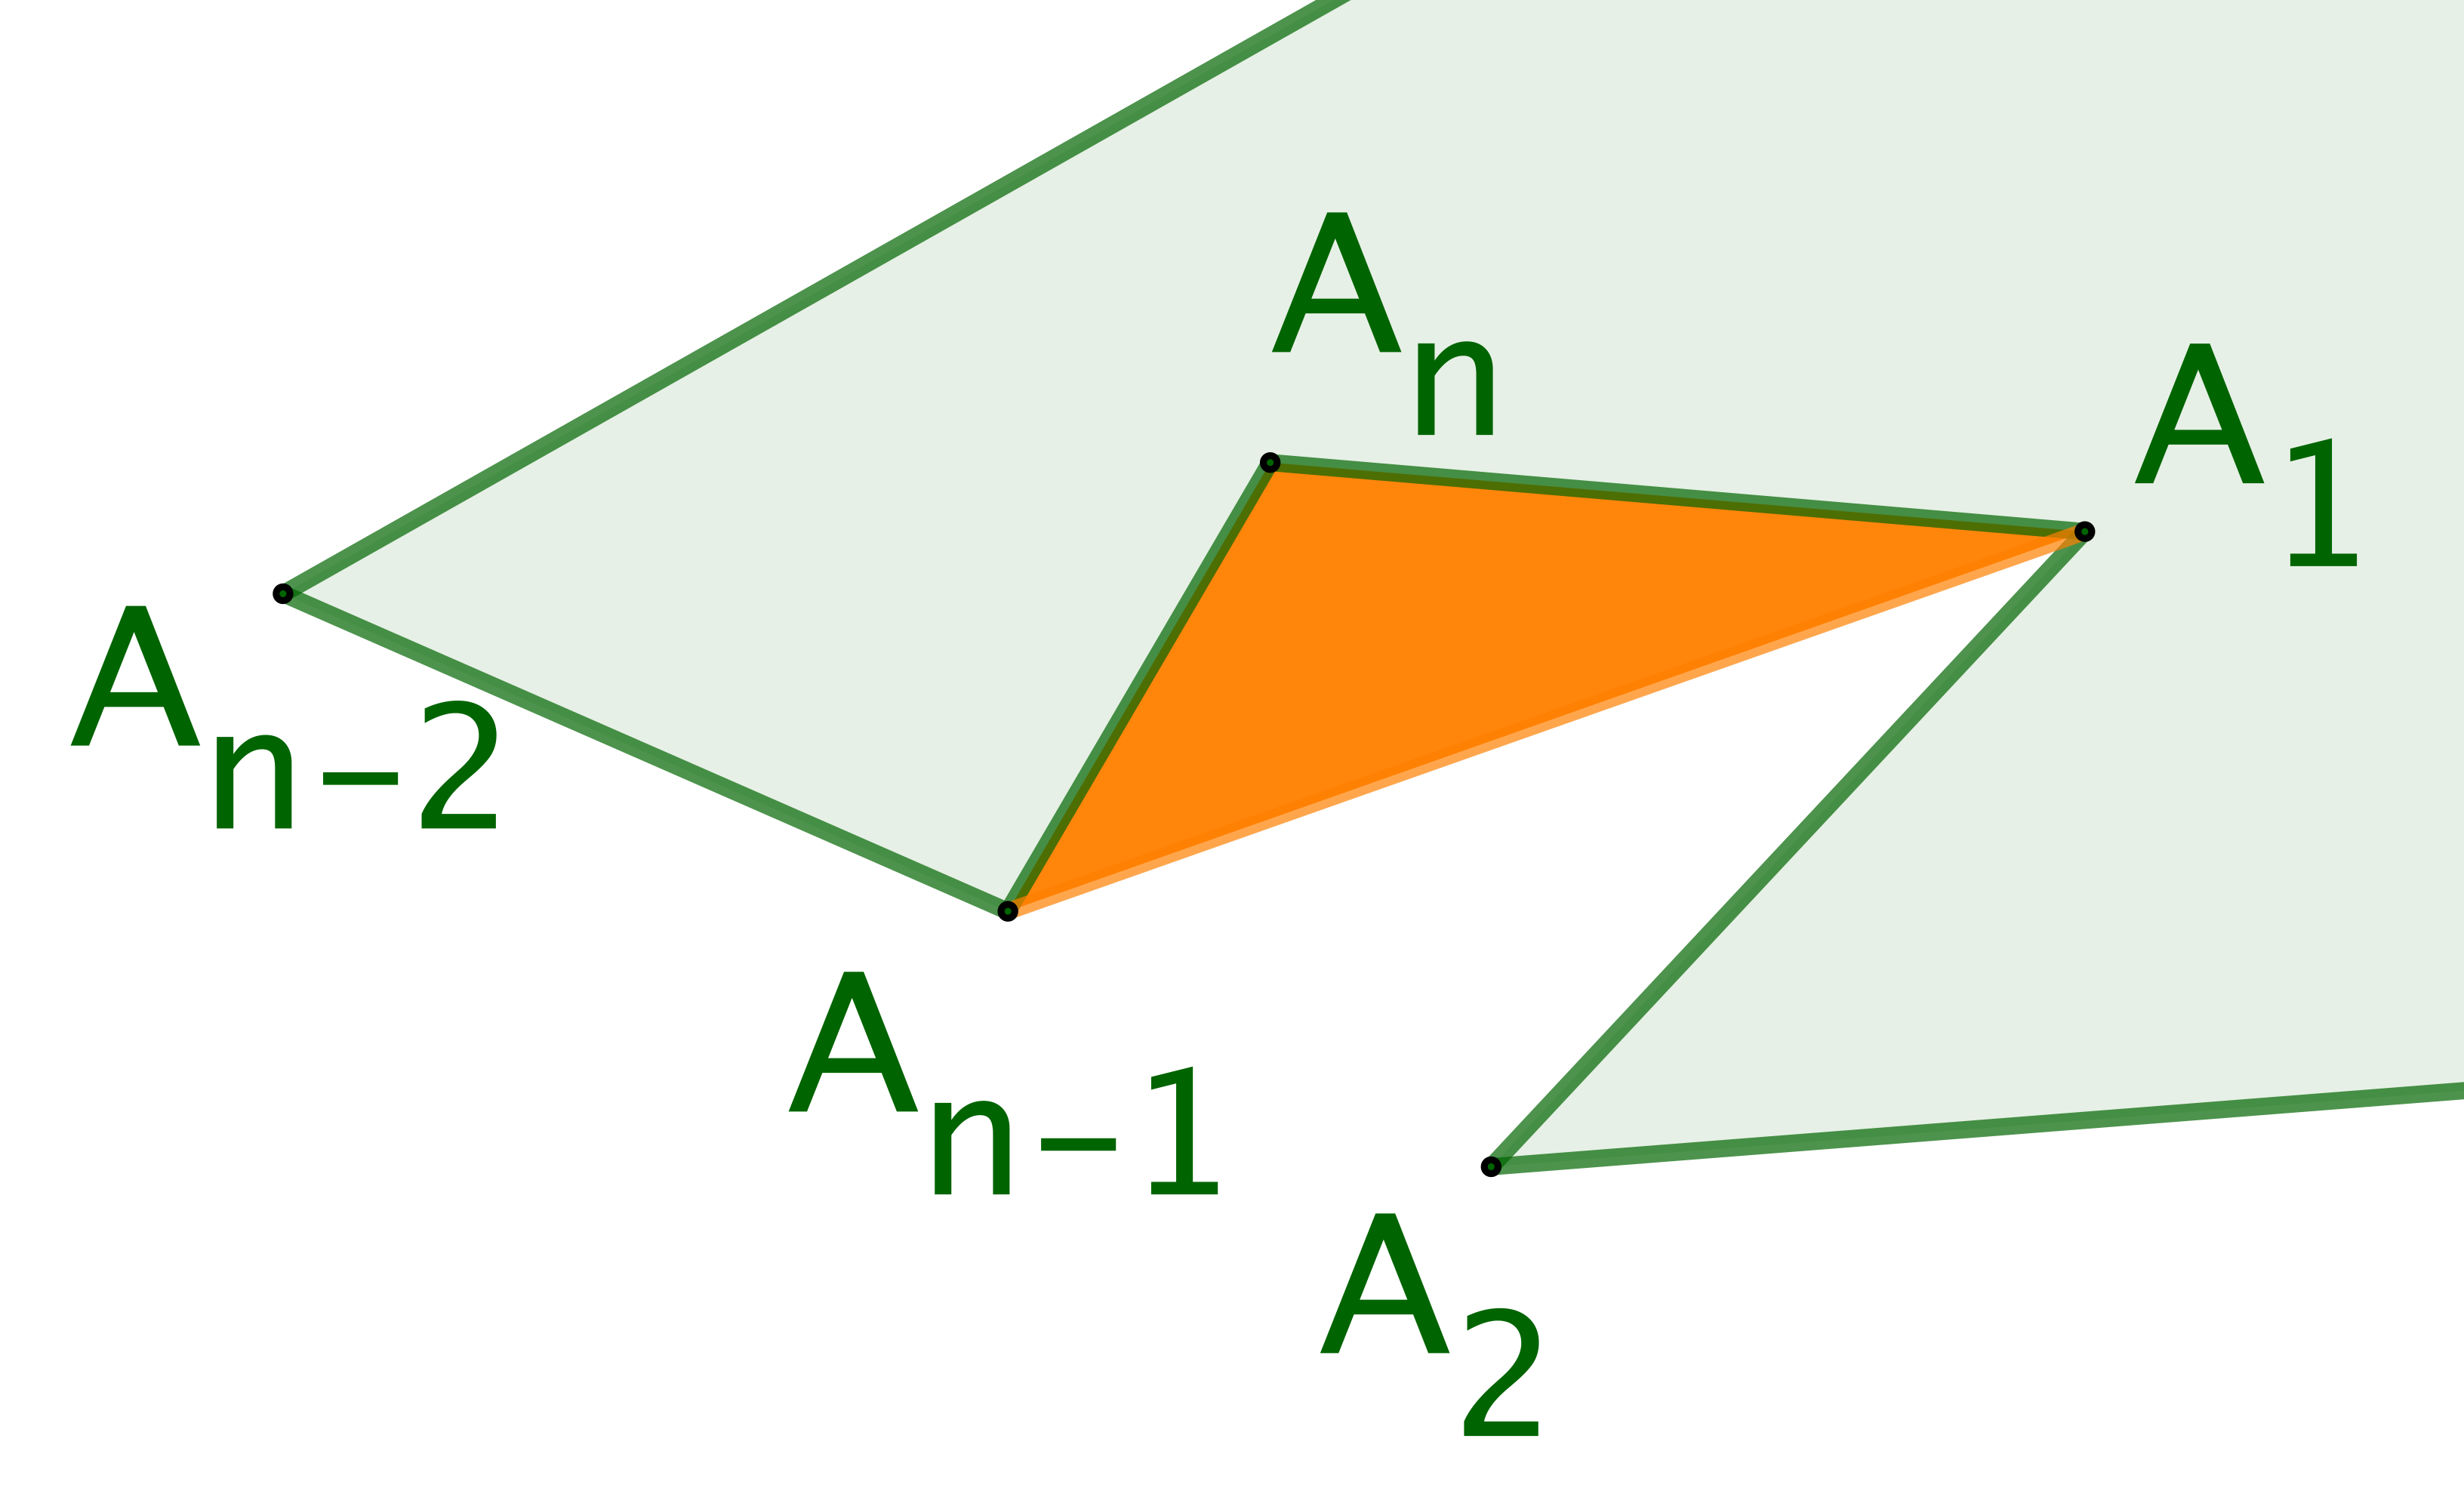
\includegraphics[scale=.4]{content/polygon/sufficient-cond/triangulation-proof-KO.png}
        
        		\smallskip
    	   		$A_{n-1} A_n A_1$ n'est pas une oreille.
    		\end{center}
    	\end{multicols}
		
		
		\noindent
		Notons $\setproba{P}^{\,\prime}$ le \kgone\ associé à la \kline\ $\setproba{L}^{\,\prime} = A_1 \cdots A_{n-1}$ où $k = n-1$ vérifie $k \in \NN_{\geq3}$. Par hypothèse, $\setproba{L}^{\,\prime}$ est positive. Nous arrivons aux calculs élémentaires suivants en utilisant $\Omega = A_1$ comme point de calcul de $\mu(\setproba{L})$.

		\leavevmode\kern-2em%
		\begin{stepcalc}[style=ar*]
			\mu(\setproba{L})
		%
%		\explnext{}
%			\dsum_{j=1}^{n} \det \big( \vect{A_1 A^{\,\prime}_j} ,  \vect{A_1 A^{\,\prime}_{j + 1}} \big)
%		%
		\explnext{}
			\dsum_{j=1}^{n-2} \det \big( \vect{A_1 A^{\,\prime}_j} ,  \vect{A_1 A^{\,\prime}_{j + 1}} \big)
			+
			\det \big( \vect{A_1 A^{\,\prime}_{n-1}} ,  \vect{A_1 A^{\,\prime}_n} \big)
			+
			\det \big( \vect{A_1 A^{\,\prime}_n} ,  \vect{A_1 A^{\,\prime}_{n+1}} \big)
		%
		\explnext*{$A_1 = A^{\,\prime}_{n+1}$ \\
		           $A_i = A^{\,\prime}_i$ \\ pour $i \leq n$}%
		          {}
			\dsum_{j=1}^{n-2} \det \big( \vect{A_1 A_j} ,  \vect{A_1 A_{j + 1}} \big)
			+
			\det \big( \vect{A_1 A_{n-1}} ,  \vect{A_1 A_n} \big)
			+
			\det \big( \vect{A_1 A_n} ,  \vect{A_1 A_1} \big)
		%
		\explnext{}
			\dsum_{j=1}^{n-2} \det \big( \vect{A_1 A_j} ,  \vect{A_1 A_{j + 1}} \big)
			+
			\det \big( \vect{A_1 A_{n-1}} ,  \vect{A_1 A_n} \big)
		%
		\explnext*{$\det \big( \vect{A_1 A_{n-1}} ,  \vect{A_1 A_1} \big) = 0$}%
		          {}
			\mu(\setproba{L}^{\,\prime})
			+
			\mu(A_{n-1} A_n A_1)
		\end{stepcalc}


		\noindent
		Par hypothèse de récurrence, nous savons que
		$\mu(\setproba{L}^{\,\prime}) \geq 0$, 
		et comme $A_{n-1} A_n A_1$ est une oreille de $\setproba{P}$, la $3$-ligne $A_{n-1} A_n A_1$ est forcément positive, d'où $\mu(A_{n-1} A_n A_1) \geq 0$ d'après le cas de base.
		Nous arrivons bien à $\mu(\setproba{L}) \geq 0$, ce qui permet de finir aisément la démonstration par récurrence.
	\end{itemize}
\end{proof}

    
% ----------------------- %


\begin{fact} \label{ngone-garea-is-area}
    Pour tout \ngone\ $\setproba{P}$, nous avons: $\garea{\setproba{P}} = \area{\setproba{P}}$.
\end{fact}


\begin{proof}
    Nous donnons juste les deux clés pour une preuve par récurrence.
    
    \begin{itemize}
		\item \textbf{Cas de base.} 
		L'égalité est immédiate pour les triangles.
	
	
		\item \textbf{Hérédité.}
		Reprenons les notations de la démonstration du fait \ref{route-direction} : $\setproba{P}$ est un \ngone\ , avec $n \in \NN_{>3}$, $\setproba{L} = A_1 A_2 \cdots A_n$ une \nline\ positive qui lui est associée, $A_{n-1} A_n A_1$ une oreille du \ngone\ $\setproba{P}$, $\setproba{P}^{\,\prime}$ le \kgone\ associé à la \kline\ $\setproba{L}^{\,\prime} = A_1 \cdots A_{n-1}$ où $k = n-1$ vérifie $k \in \NN_{\geq3}$, avec $\setproba{L}^{\,\prime}$ positive. Nous arrivons aux calculs élémentaires suivants.

		\leavevmode\kern-2em%
		\begin{stepcalc}[style=ar*]
			\area{\setproba{P}}
		%
		\explnext*{$A_{n-1} A_n A_1$ est une oreille de $\setproba{P}$.}%
		          {}
		    \area{\setproba{P}^{\,\prime}} + \area{A_{n-1} A_n A_1}
		%
		\explnext*{Hypothèse de récurrence et cas de base.}%
		          {}
		    \garea{\setproba{P}^{\,\prime}} + \garea{A_{n-1} A_n A_1}
		%
		\explnext*{Voir le fait \ref{route-direction}.}%
		          {}
		    \frac12 \big( \mu(\setproba{L}^{\,\prime}) + \mu(A_{n-1} A_n A_1) \big)
		%
		\explnext*{Comme dans la preuve du fait \ref{route-direction}.}%
		          {}
		    \frac12 \mu(\setproba{L})
		%
		\explnext*{Voir le fait \ref{route-direction}.}%
		          {}
		    \garea{\setproba{P}}
		\end{stepcalc}
    \end{itemize}
\end{proof}


% ----------------------- %


\begin{fact} \label{no-cross-max}
    Si une \nline\ $\setproba{L}$ non dégénérée n'est pas un \ngone, donc est un polygone croisé, alors on peut construire une \nline\ $\setproba{L}^{\,\prime}$ telle que 
	$\perim{\setproba{L}^{\,\prime}} = \perim{\setproba{L}}$ 
	et 
	$\garea{\setproba{L}^{\,\prime}} > \garea{\setproba{L}}$.
\end{fact}


\begin{proof}
	L'idée est simple: comme nous savons que les triangles $A^{\,\prime}_i A^{\,\prime}_{i+1} A^{\,\prime}_{i+2}$ ne sont pas tous orientés de la même façon, il suffit de remplacer l'un de ces triangles par son symétrique relativement à la droite $( A^{\,\prime}_i A^{\,\prime}_{i+2} )$ pour diminuer ou augmenter $\mu(\setproba{L})$ suivant le signe initial de $\mu(\setproba{L})$.
	Les figures suivantes illustrent cette idée que nous formalisons juste après
	(les nombres indiquées sont les aires calculées par \geogebra).
	
    \begin{multicols}{3}
    	\small\itshape
	
        \foreach \i/\t in {1/{Valeur initiale}, 2/{Coup perdant}, 3/{Coup gagnant}} {
	        \begin{center}
    	    	\includegraphics[scale=.35]{content/polygon/sufficient-cond/no-cross-max-\i.png}
	
				\smallskip
				\t.
        	\end{center}
        }
    \end{multicols}
        
    Supposons pour commencer que $\mu(\setproba{L}) \leq 0$. Dans ce cas, considérons $A^{\,\prime}_i A^{\,\prime}_{i+1} A^{\,\prime}_{i+2}$ orienté positivement, autrement tel que
    $\delta = \det \big( \vect{A^{\,\prime}_i A^{\,\prime}_{i+1}} , \vect{A^{\,\prime}_i A^{\,\prime}_{i+2}} \big) > 0$.
    En calculant $\mu(\setproba{L})$ via $\Omega = A^{\,\prime}_i$, la somme des déterminants de la définition contient $\delta$.
    En remplaçant $A^{\,\prime}_i A^{\,\prime}_{i+1} A^{\,\prime}_{i+2}$ par son symétrique relativement à la droite $( A^{\,\prime}_i A^{\,\prime}_{i+2} )$, nous obtenons une nouvelle \nline\ $\setproba{L}^{\,\prime}$ telle que le calcul de $\mu(\setproba{L}^{\,\prime})$ se fait en remplaçant $\delta$ par $(- \delta)$ dans la définition de $\mu(\setproba{L})$.
    Nous avons alors $\mu(\setproba{L}^{\,\prime}) < \mu(\setproba{L}) \leq 0$, et donc
   	$\garea{\setproba{L}^{\,\prime}} > \garea{\setproba{L}}$ en appliquant la valeur absolue.
    Comme $\perim{\setproba{L}^{\,\prime}} = \perim{\setproba{L}}$, clairement, le contrat est rempli dès que $\mu(\setproba{L}) \leq 0$.
    
    Si $\mu(\setproba{L}) > 0$, la démarche est similaire, mais via un triangle orienté négativement.
\end{proof}


% ----------------------- %


\begin{fact} \label{suff-cond}
    Soit $n \in \NN_{\geq3}$ un naturel fixé.
    Considérons tous les \ngones\ de périmètre fixé. Parmi tous ces \ngones, il en existe au moins un d'aire maximale.
\end{fact}


\begin{proof}
	Ce qui suit nous donne plus généralement l'existence d'un \ngone, au moins, maximisant l'aire généralisée parmi toutes les \nlines\ de périmètre fixé $p$. Ce résultat plus fort convient d'après le fait \ref{ngone-garea-is-area}.
    %    
    \begin{itemize}
        \item On munit le plan d'un repère orthonormé direct $\pvaxes{O | i | j}$. 


        \item On note $\setproba{Z}$ l'ensemble des \nlines\ $\setproba{L} = A_1 A_2 \cdots A_n$ telles que
        $\perim{A_1 A_2 \cdots A_n} = p$
        et
        $A_1\coord{0 | 0}$.%
        \footnote{
        	Le mot \og \emph{Zeile} \fg\ est une traduction possible de \og \emph{ligne} \fg\ en allemand.
        }


        \item Considérons alors $\setproba{G} \subset \RR^{2n}$ l'ensemble des uplets $\big( x(A_1) ; y(A_1) ; \dots ; x(A_n) ; y(A_n) \big)$ correspondant aux coordonnées des sommets $A_i$ de \nlines\ appartenant à $\setproba{Z}$.
        
        
        \item $\setproba{G}$ est clairement fermé dans $\RR^{2n}$.
        De plus, il est borné, car les coordonnées des sommets des \nlines\ considérées le sont.        
        En résumé, $\setproba{G}$ est un compact de $\RR^{2n}$.


        \item Nous définissons la fonction $s: \setproba{G} \rightarrow \RRp$ qui à un uplet de $\setproba{G}$ associe l'aire généralisée de la \nline\ qu'il représente. 
        Cette fonction est continue comme valeur absolue d'une fonction polynomiale en les coordonnées.
       
        
        \item Finalement, par continuité et compacité, on sait que $s$ admet un maximum sur $\setproba{G}$.
        Or, un tel maximum ne peut être atteint en une \nline\ dégénérée, clairement, ni en un polygone croisé d'après le fait \ref{no-cross-max}, donc un tel maximum sera obtenu en un \ngone. That's all folks!
    \end{itemize}    
\end{proof}


% ----------------------- %


\begin{fact}
    Soit $n \in \NN_{\geq3}$ un naturel fixé.
    Considérons tous les \ngones\  de périmètre fixé. Parmi tous ces \ngones, un seul est d'aire maximale, c'est le \ngone\ régulier.
\end{fact}


\begin{proof}
    Ceci découle directement des faits \ref{nece-cond} et \ref{suff-cond}.
    Ici s'achève notre joli voyage.
\end{proof}